\documentclass[11pt]{amsart}
%\usepackage[english]{babel}
\usepackage{appendix}
\usepackage{amsmath}
\usepackage{amsfonts}
\usepackage{amssymb}
%\usepackage{showlabels}
\usepackage{amsthm}
\usepackage{marginnote}
\usepackage{stmaryrd}
\usepackage{enumitem}
\usepackage[english]{babel}
\usepackage{yfonts}
\usepackage[T1]{fontenc}
\usepackage[utf8x]{inputenc}
%\usepackage{enumerate}
\usepackage{verbatim}
\usepackage{graphicx}
\usepackage{verbatim}
\usepackage{faktor}
\usepackage{xcolor}
\usepackage{xfrac}
\usepackage{tikz,tikz-cd}
\usepackage[all]{xy}
\usepackage{bbm}

\newcommand{\M}[4]{\overline{\mathcal M}_{#1,#2}(#3,#4)}
\newcommand{\Q}[4]{\overline{\mathcal Q}_{#1,#2}(#3,#4)}
\newcommand{\Qe}[4]{\overline{\mathcal Q}^{\epsilon}_{#1,#2}(#3,#4)}
\newcommand{\Qt}[4]{\widetilde{\mathcal Q}_{#1,#2}(#3,#4)}
\newcommand{\QG}[4]{\overline{\mathcal QG}_{#1,#2}(#3,#4)}
\newcommand{\QGe}[4]{\overline{\mathcal QG}^{\epsilon}_{#1,#2}(#3,#4)}
\newcommand{\PP}{\mathbb P}
\newcommand{\Z}{\mathbb{Z}}
\newcommand{\N}{\mathbb{N}}
\newcommand{\OO}{\mathcal{O}}
\renewcommand{\to}{\rightarrow}
\newcommand{\A}{\mathcal A}
\newcommand{\B}{\mathcal B}
\newcommand{\C}{\mathfrak C}
\renewcommand{\L}{\mathcal L}
\newcommand{\MM}{\mathfrak M}
\newcommand{\Aaff}{\mathbb{A}}
\newcommand{\kfield}{\mathbb{K}}
\newcommand{\comp}{\chi}
\newcommand{\sst}{\sigma^{ss}}
\newcommand{\Pic}{\operatorname{Pic}}
\newcommand{\Def}{\operatorname{Def}}
\newcommand{\Spec}{\operatorname{Spec}}
\newcommand{\Proj}{\operatorname{Proj}}
\newcommand{\Hom}{\operatorname{Hom}}
\newcommand{\Ext}{\operatorname{Ext}}
\newcommand{\Gm}{\mathbb{G}_m}
\newcommand{\virt}[1]{[#1]^{\operatorname{virt}}}
\newcommand{\Id}{\operatorname{Id}}
\newcommand{\CC}{\mathbb{C}}
\newcommand{\QQ}{\mathbb{Q}}
\newcommand{\HH}{\operatorname{H}}
\newcommand{\Achow}{\operatorname{A}}

\newcommand{\bq}{\begin{equation}}
\newcommand{\eq}{\end{equation}}
\newcommand{\ba}{\begin{aligned}}
\newcommand{\ea}{\end{aligned}}
\newcommand{\be}{\begin{enumerate}}
\newcommand{\ee}{\end{enumerate}}
\newcommand{\bsm}{\left(\begin{smallmatrix}}
\newcommand{\esm}{\end{smallmatrix}\right)}                   
\newcommand{\bpm}{\begin{pmatrix}}
\newcommand{\epm}{\end{pmatrix}}
\newcommand{\barr}{\begin{displaymath}\begin{array}{cccc}}
\newcommand{\earr}{\end{array}\end{displaymath}}
\newcommand{\barrl}{\begin{displaymath}\begin{array}{lcl}}
\newcommand{\earrl}{\end{array}\end{displaymath}}
\newcommand{\barl}{\begin{displaymath}\begin{array}{l}}
\newcommand{\earl}{\end{array}\end{displaymath}}
\newcommand{\bxym}{ \begin{displaymath}\xymatrix }
\newcommand{\exym}{\end{displaymath}}
\newcommand{\bcd}{\begin{center}\begin{tikzcd}}
\newcommand{\ecd}{\end{tikzcd}\end{center}}
\newcommand{\R}{\operatorname{R}^{\bullet}}
%\newcommand{\sslash}{\mathbin{/\mkern-6mu/}}
\newcommand{\tr}{{\rm tr}}
\newcommand{\Isom}{\text{Isom}}
\newcommand{\pr}{\operatorname{pr}}
\newcommand{\ev}{\operatorname{ev}}
\newcommand{\codim}{\operatorname{codim}}
\newcommand{\vdim}{\operatorname{vdim}}
\newcommand{\ildef}[1]{\textbf{\textsc{#1}}}
\newcommand{\om}[1]{\overline{\mathcal{#1}}}
\newcommand{\h}{\operatorname{h}}

\theoremstyle{plain}
\newtheorem{thm}{Theorem}[section]
\newtheorem{lem}[thm]{Lemma}
\newtheorem{lemma}[thm]{Lemma}
\newtheorem{prop}[thm]{Proposition}
\newtheorem{cor}[thm]{Corollary}
\newtheorem*{teo*}{Theorem}
\newtheorem{ipotesi}{ipotesi}
\newtheorem*{nota}{Nota}
\newtheorem{claim}{Claim}
\newtheorem{question}[thm]{Question}
\newtheorem{conj}[thm]{Conjecture}

\theoremstyle{definition}
\newtheorem{example}[thm]{Example}
\newtheorem{ex}[thm]{Example}
\newtheorem{dfn}[thm]{Definition}
\newtheorem{definition}[thm]{Definition}
\newtheorem{aside}[thm]{Aside}
\newtheorem{remark}[thm]{Remark}
\newtheorem{com}[thm]{Comment}
\newtheorem{num}{Number}
\newtheorem*{sketch}{Sketch}
\newtheorem*{rem}{Remark}
\newtheorem*{aside*}{Aside}
\newtheorem*{acknowledgements}{Acknowledgements}

\newcommand{\ilemph}[1]{\textbf{\textsc{#1}}}


\setcounter{tocdepth}{1}

\newcommand{\todo}[1]{\vspace{5mm}\par \noindent
\framebox{\begin{minipage}[c]{0.95 \textwidth} \tt #1\end{minipage}} \vspace{5mm} \par}

\def\ti{-\allowhyphens}
\newcommand{\thismonth}{\ifcase\month % case 0 --- impossible!
  \or January\or February\or March\or April\or May\or June%
  \or July\or August\or September\or October\or November%
  \or December\fi}
\newcommand{\thismonthyear}{{\thismonth} {\number\year}}
\newcommand{\thisdaymonthyear}{{\number\day} {\thismonth} {\number\year}}

\usepackage[T1]{fontenc}
\usepackage{newpxtext,newpxmath}

\title{A Quantum Lefschetz Theorem for Quasimap Invariants via Relative Quasimaps}
\author{Luca Battistella and Navid Nabijou}
\begin{document}

\begin{abstract}
\end{abstract}

\maketitle
\appendixtitletocoff
\tableofcontents

\section{Introduction}

\subsection{Stable quasimaps}
The moduli space of \ilemph{stable toric quasimaps}
\begin{equation*} \Q{g}{n}{X}{\beta} \end{equation*}
was constructed by Ciocan-Fontanine and Kim \cite{CF-K} as an alternative compactification of the moduli space of smooth curves in a toric variety $X$. It is a Deligne--Mumford stack of finite type, and is proper if $X$ is proper. Moreover, when $X$ is smooth it admits a perfect obstruction theory and hence a virtual fundamental class, which one can use to define curve-counting invariants for $X$, called \ilemph{quasimap invariants}.

This theory agrees with the theory of stable quotients \cite{MOP} when both are defined, namely when $X$ is a projective space.  There is a common generalisation given by the theory of stable quasimaps to GIT quotients \cite{CFKM}. For simplicity we will work in the toric setting (though this restriction is probably not essential for our arguments). Thus when we say ``quasimap'' we are implicitly talking about toric quasimaps.

The quasimap invariants are expected to coincide with the Gromov--Witten invariants when $X$ is a toric Fano variety \cite{CM}; this is known to hold when $X=\PP^N$ as well as in a number of other cases.

In general, however, the invariants differ, the difference being encoded by certain wall-crossing formulas \cite{CF-K-wallcrossing}. The motivation for this comes from mirror symmetry: the idea is that the quasimap invariants of $X$ should correspond to the $B$-side theory of $X$ (this is in contrast to the Gromov--Witten invariants, which live on the $A$-side); see \cite[\S 7]{CF-K}.

\subsection{Relative stable maps}
In \cite{Ga} Gathmann consructs a moduli space of relative stable maps to the pair $(X,Y)$ as a closed substack of the moduli space of (absolute) stable maps to $X$:
\begin{equation*} \M{g}{\alpha}{X|Y}{\beta} \hookrightarrow \M{g}{n}{X}{\beta} \end{equation*}
Unfortunately this space does not admit a natural perfect obstruction theory; nevertheless in the case where $Y$ is very ample it is still possible to construct a virtual fundamental class on the moduli space, and hence to define relative Gromov--Witten invariants.

Gathmann then proves a recursion formula which allows one to recover the relative Gromov--Witten invariants from the absolute ones. This is  applied in \cite{Ga-MF} to obtain a quantum Lefschetz theorem for $Y \subseteq X$.

\subsection{Relative stable quasimaps}
In this paper we combine the two stories above, constructing moduli spaces of relative stable quasimaps. We prove a recursion relation similar to Gathmann's formula, and use this to derive a quantum Lefschetz formula for quasimap invariants.

The plan of the paper is as follows. In \S\S \ref{Subsection stable quasimaps}-\ref{Subsection relative stable maps} we provide a brief review of the theories of stable quasimaps and relative stable maps mentioned above. Then in \S \ref{Subsection relative stable quasimaps} we define the moduli spaces of relative stable quasimaps
\begin{equation*} \Q{g}{\alpha}{X|Y}{\beta} \end{equation*}
where $X$ is a smooth toric variety and $Y$ is a smooth hypersurface. We do not require that $Y$ is toric, although we do assume it is rationally equivalent to a non-negative linear combination of toric hypersurfaces.

In \S \ref{Section recursion for PN} we examine the special case of $H \subseteq \PP^N$. We find that, although the moduli space is not in general smooth, it is irreducible of the expected dimension (in fact, more than this: it is the closure of the so-called ``nice locus''). Thus it admits a fundamental class which we can use to define relative quasimap invariants.

For $\PP^N$ there exists a comparison morphism from the moduli space of stable maps to the moduli space of quasimaps, which is birational. We use this morphism to push down Gathmann's recursion formula for relative stable maps to obtain a recursion formula for relative stable quasimaps. The stronger stability condition for quasimaps significantly simplifies the correction terms which appear.

In \S \ref{Section recursion formula in general case} we extend the recursion formula to arbitrary pairs $(X,Y)$ where $Y$ is very ample, by taking the embedding $X \hookrightarrow \PP^N$ defined by $\OO(Y)$ and pulling back the formula for $(\PP^N,H)$. This of course requires some comparison theorems for virtual classes, which requires us to examine the perfect obstruction theories.

In \S \ref{Section quasimap mirror theorem} we apply the recursion formula obtained in \S \ref{Section recursion formula in general case} to obtain a quantum Lefschetz theorem for quasimap invariants. This recovers [REFERENCE] in \cite{CF-K-wallcrossing}.

We also include several appendices, collecting together results which are presumably well-known to experts, but which we could not find references for in the literature.

Appendix [REF] contains foundational lemmas of quasimap theory, including functoriality, the existence of relative perfect obstruction theories and the splitting theorem.

Appendix [REF] discusses a well-known intersection-theoretic construction -- the so-called ``diagonal pullback'' -- and shows that it agrees with the virtual pullback of \cite{Manolache-Pull} when both are defined.

Finally Appendix [REF] discusses the comparison morphism from maps to quasimaps (used in the proof of the recursion relation in \S \ref{Section recursion for PN}).

\begin{acknowledgements} The authors wish to thank Cristina Manolache for many helpful discussions. L.B. is supported by [REF] and N.N. is supported by [REF]
\end{acknowledgements}

\subsection{Table of notation}













\section{Relative stable quasimaps} \label{Section relative stable quasimaps}

\subsection{Review of absolute stable quasimaps} \label{Subsection stable quasimaps}
We briefly recall the definition and basic properties of the moduli space of toric quasimaps; see \cite{CF-K} for more details.
\begin{definition}[{\cite[Definition 3.1.1]{CF-K}}] Let $X= X_{\Sigma}$ be a smooth and projective toric variety with fan $\Sigma \subseteq N_{\QQ}$, let $M = N^\vee = \Hom(N,\Z)$ and let $\OO_{X_\Sigma}(1)$ be a fixed polarisation, which we can write (non-uniquely) in terms of the $T$-invariant divisors as:
\begin{equation*} \OO_{X_\Sigma}(1) = \otimes_{\rho \in \Sigma(1)} \OO_{X_\Sigma}(D_\rho)^{\otimes \alpha_\rho} \end{equation*}
for some $\alpha_\rho \in \Z$. We fix the following numerical invariants: a genus $g \geq 0$, number of marked points $n \geq 0$ and effective curve class $\beta \in \HH_2^+(X)$. Then a \ilemph{stable (toric) quasimap} is given by the data
\begin{equation*} ((C,x_1,\ldots,x_n), (L_\rho,u_\rho)_{\rho \in \Sigma(1)}, (\varphi_m)_{m \in M}) \end{equation*}
where:
\begin{enumerate}
\item $(C,x_1,\ldots,x_n)$ is a prestable curve of genus $g$ with $n$ marked points;
\item the $L_\rho$ are line bundles on $C$ of degree $d_\rho = D_\rho \cdot \beta$;
\item the $u_\rho$ are global sections of $L_\rho$;
\item $\varphi_m \colon \bigotimes_{\rho \in \Sigma(1)} L_\rho^{\otimes \langle \rho, m \rangle} \to \OO_C$ are isomorphisms, such that $\varphi_{m} \otimes \varphi_{m^\prime} = \varphi_{m + m^\prime}$ for all $m, m^\prime \in M$.
\end{enumerate}
These are required to satisfy the following two conditions:
\begin{enumerate}
\item \ilemph{nondegeneracy}: there is a finite (possibly empty) set of smooth and non-marked points $B \subseteq C$, called the \ilemph{basepoints} of the quasimap, such that for all $x \in C \setminus B$ there exists a maximal cone $\sigma \in \Sigma_{\operatorname{max}}$ with $u_\rho(x) \neq 0$ for all $\rho \not\subset \sigma$;
\item \ilemph{stability}: if we let $L = \otimes_\rho L_\rho^{\otimes \alpha_\rho}$ then the following $\QQ$-divisor is ample
\begin{equation*} \omega_C(x_1 + \ldots + x_n)\otimes L^{\otimes \epsilon} \end{equation*}
for every rational $\epsilon > 0$.
\end{enumerate}
\end{definition}
It can be shown that this definition does not depend on the choice of polarisation.

\begin{remark} This definition is motivated by D. Cox's description of the functor of points of a toric variety in terms of $\Sigma$-collections \cite{CoxFunctor}; see also Appendix \ref{Functoriality of Quasimap Spaces Section}. A quasimap defines a rational map $C \dashrightarrow X$ with base locus equal to $B$. (This can be expressed in a more generalisable manner as follows: a quasimap is a map to the stack quotient $[\mathbb{A}^{\Sigma(1)} / (\Gm)^r]$ such that $B$ is the preimage of the unstable locus.)

In particular a quasimap without any basepoints defines a morphism $C \to X$. Thus the basepoints appear in the (virtual) boundary of the moduli space, in much the same way as the locus of stable maps with rational tails appears in the boundary of the moduli space of stable maps. This is something more than just a vague analogy; these loci correspond to each other under the comparison morphism when $X\simeq\PP^N$; see Appendix \ref{Section comparison morphism}. \end{remark}

More generally, we can define the notion of a family of quasimaps over a base scheme $S$, and what it means for two such families to be isomorphic; we thus obtain a moduli space
\begin{equation*} \Q{g}{n}{X}{\beta} \end{equation*}
of stable (toric) quasimaps to $X$, which is a proper Deligne--Mumford stack of finite type.


As with the case of stable maps, there is a combinatorial characterisation of stability which is much easier to check in practice; a prestable quasimap is stable if and only if the following conditions hold:
\begin{enumerate}
\item the line bundle $L$ defined above must have strictly positive degree on any rational component with fewer than three special points, and on any elliptic component with no special points;
\item $C$ cannot have any rational components with fewer than two special points (called \emph{rational tails}).
\end{enumerate}
Condition (1) is analogous to the ordinary stability condition for stable maps. Condition (2) is new, however, and gives quasimaps a distinctly different flavour to stable maps; we shall sometimes refer to it as the \ilemph{strong stability condition}. 

%\begin{remark}
% Notice that quasimap spaces are ``smaller'', so if a comparison morphism exists it should be from stable maps to quasimaps; in fact a morphism between the moduli spaces comes with a morphism of the universal curves, and this ought to be a contraction of the rational tails (the other way round, one could sprout a rational tail from any base points, and maybe even the degree of the line bundles would be determined, but a fundamental indeterminacy remains as to what the sections should be, i.e. where does the rational tail map).
%\end{remark}

\begin{remark} Unlike in Gromov--Witten theory, $\Q{g}{n+1}{X}{\beta}$ is \emph{not} the universal curve over $\Q{g}{n}{X}{\beta}$ since markings cannot be basepoints. In fact there is not even a morphism between these spaces in general.\end{remark}
%Instead, the universal curve $\mathcal C_{g,n}^\mathcal{Q}$ is a substack of $\MM_{g,n+1}(X,\beta)$ and comparing the geometry of $\om{Q}_{g,n+1}$ and $\mathcal{C}^{\mathcal{Q}}_{g,n}$ results in \emph{string transformations} that determine the difference between generating functions for $\epsilon_1$- and $\epsilon_2$-stable quasimaps \cite[\S 6 and 7]{CF-K-wallcrossing}.

The moduli space $\Q{g}{n}{X}{\beta}$ admits a perfect obstruction theory relative to the moduli space $\MM_{g,n}$ of source curves, and hence one can construct a virtual class
\begin{equation*} \virt{\Q{g}{n}{X}{\beta}} \in \Achow_{\operatorname{vdim}\Q{g}{n}{X}{\beta}} \left( \Q{g}{n}{X}{\beta} \right) \end{equation*}
where the virtual dimension is the same as for stable maps:
\begin{equation*} \operatorname{vdim}\Q{g}{n}{X}{\beta} = (\dim{X} - 3)(1-g) - (K_X \cdot \beta) + n \end{equation*}
Since the markings are not basepoints there exist evaluation maps
\begin{equation*} \ev_i : \Q{g}{n}{X}{\beta} \to X \end{equation*}
and there are $\psi$-classes defined in the usual way by pulling back the relative dualising sheaf of the universal curve
\begin{equation*} \psi_i = \operatorname{c}_1(x_i^* \omega_{\mathcal{C}/\om{Q}}) \end{equation*}
where $\mathcal{C} \to \om{Q} = \Q{g}{n}{X}{\beta}$ is the universal curve and $x_i : \om{Q} \to \mathcal{C}$ is the section defining the $i$th marked point. Putting all these pieces together, we can define \ilemph{quasimap invariants}:
\begin{equation*} \langle \gamma_1 \psi^{a_1} , \ldots, \gamma_n \psi^{a_n} \rangle_{g,n,\beta}^X = \int_{\virt{\Q{g}{n}{X}{\beta}}} \prod_{i=1}^n \ev_i^* (\gamma_i) \psi_i^{a_i} \end{equation*}
We use the same correlator notation as in Gromov--Witten theory; this should not cause any confusion.

[EXAMPLE: $\Q{0}{2}{\PP^2}{1}$ and $\M{0}{2}{\PP^2}{1}$]

\begin{remark}
 There is a more general notion of \ilemph{$\epsilon$-stable quasimap} \cite[\S 7.1]{CFKM}. The stability condition, namely that the line bundle
\begin{equation*} \omega_C(x_1 + \ldots + x_n)\otimes L^{\otimes \epsilon} \end{equation*} 
is ample, is required to hold for a single fixed $\epsilon \in \QQ_{>0}$ (instead of for arbitrary $\epsilon$, as was the case for stable quasimaps).

This has the effect of allowing some rational tails to appear, as long as their degree is high enough with respect to $\epsilon$. In order to keep the moduli space separated, one has to bound the multiplicity of the basepoints that can occur.

By boundedness and the fact that the degree is an integer-valued function, it follows that there exist finitely many critical values of $\epsilon$ which divide $\QQ_{>0}$ into chambers inside which the moduli spaces $\Qe{g}{n}{X}{\beta}$ do not change.

Furthermore, the limiting values $\epsilon=+\infty$ and $\epsilon=0^+$ recover the moduli spaces of stable maps and (ordinary) quasimaps respectively. As such the moduli spaces $\Qe{g}{n}{X}{\beta}$ are meant to interpolate between the two, and they have proven particularly successful as a tool to compare the resulting invariants \cite{CF-K-wallcrossing}.
\end{remark}

\begin{remark}
There is another variant which is going to play a role in later sections: that of \emph{parametrised quasimaps} \cite[\S 7]{CF-K}. The idea is that a parametrised quasimap comes with a preferred rational component (by introducing the extra data of an isomorphism with $\PP^1$) and the stability condition is imposed \emph{on all but the preferred component}. This mimics the construction of graph spaces in Gromov-Witten theory and induces a $\Gm$-action on $\QG{g}{n}{X}{\beta}$ by rotating the preferred component. The fixed loci and equivariant normal bundle are well-understood, at least in the toric setting \cite[\S 7]{CF-K}.
 
Note that we do not require $2g-2+n\geq 0$ anymore, due to the modified stability condition. In particular it makes sense, and turns out to be very useful, to consider unmarked parametrised quasimaps $\QG{0}{0}{X}{\beta}$. In this case the source curve needs to be irreducible. 
\end{remark}

\begin{example} $\QG{0}{0}{\PP^r}{d} = \PP^N$ with $N=(r+1)(d+1)-1$. Indeed, the curve and line bundle must be $(\PP^1,\mathcal O_{\PP^1}(d))$ and we are left with choosing $r+1$ sections of $\mathcal O_{\PP^1}(d)$ (not all zero) up to automorphisms of $\mathcal O_{\PP^1}(d)$, i.e. up to scaling. See e.g. \cite{Bertram} for an early appearance of such spaces.\end{example}

\subsection{Review of relative stable maps} \label{Subsection relative stable maps} Given a smooth projective variety $X$ and a smooth divisor $Y$, the moduli space of relative stable maps parametrises stable maps to $X$ with specified tangencies to $Y$ at the marked points; see \cite{Ga} for details.

\begin{definition}[{\cite[Definition 1.1]{Ga}}] Let $X$ be a smooth projective variety and $Y \subseteq X$ a smooth divisor. Fix a number $n \geq 0$ of marked points, a curve class $\beta \in \HH_2^+(X)$ and an $n$-tuple $\alpha = (\alpha_1, \ldots, \alpha_n)$ of non-negative integers such that $\Sigma_i \alpha_i \leq Y \cdot \beta$. Then the moduli space
\begin{equation*} \M{0}{\alpha}{X|Y}{\beta} \end{equation*}
of relative stable maps to $(X,Y)$ is defined to be the locus in $\M{0}{n}{X}{\beta}$ of stable maps $(C \to S , (x_i : S \to C)_{i=1}^n , f : C \to X)$ satisfying the following two conditions:
\begin{enumerate}
\item if $x_i$ is a marked point such that $\alpha_i > 0$ then $f(x_i) \in Y$;
\item if we consider $f^* [Y] \in \Achow_0(f^{-1}Y)$ then the difference $f^* [Y] - \Sigma_i \alpha_i x_i$ is an effective class.
\end{enumerate}
This forms a closed substack of $\M{0}{n}{X}{\beta}$. Condition (1) is required in order for the class $\Sigma_i \alpha_i x_i$ to make sense in $\Achow_0(f^{-1}Y)$.
\end{definition}

\begin{remark} The definition above works in families; however there is a more combinatorial definition for individual maps which is more useful in practice (see \cite[Remark 1.4]{Ga}): a stable map $(C,x_1, \ldots, x_n,f)$ is a relative stable map if and only if, if $Z$ is a connected component of $f^{-1}(Y) \subseteq C$, then
\begin{enumerate}
\item if $Z$ is a point and is equal to a marked point $x_i$, then the multiplicity of $f$ to $Y$ at $x_i$ is greater than or equal to $\alpha_i$;
\item if $Z$ is one-dimensional (hence a union of irreducible components of $C$) and if we let $C^{(i)}$ for $1 \leq i \leq r$ denote the irreducible components of $C$ adjacent to $Z$, and $m^{(i)}$ denote the multiplicity of $f|_{C^{(i)}}$ to $Y$ at the node $Z \cap C^{(i)}$, then we must have:
\begin{equation} \label{Inequality relative stable maps} Y \cdot f_* [Z] + \sum_{i=1}^r m^{(i)} \geq \sum_{x_i \in Z} \alpha_i \end{equation}
\end{enumerate} \end{remark}

\begin{remark} In the case of maximal multiplicity $\Sigma_{i} \alpha_i = Y \cdot \beta$, all the inequalities in the above definition must actually be equalities. \end{remark}

In the case $X=\PP^N$, $Y=H$ one can show that $\M{0}{\alpha}{\PP^N|H}{d}$ is irreducible with dimension equal to the expected dimension:
\begin{equation*} \vdim \M{0}{\alpha}{X|Y}{\beta} = \vdim{\M{0}{n}{X}{\beta}} - \sum_i \alpha_i \end{equation*}
Hence it has a fundamental class from which one can define relative Gromov--Witten invariants.

In general if $Y \subseteq X$ is very ample one can use the embedding $X \hookrightarrow \PP^N$ to obtain a cartesian diagram:
\bcd
\M{0}{\alpha}{X|Y}{\beta} \ar[r] \ar[d] \ar[rd,phantom,"\square"] & \M{0}{\alpha}{\PP^N|H}{d} \ar[d] \\
\M{0}{n}{X}{\beta} \ar[r,"\varphi"] & \M{0}{n}{\PP^N}{d}
\ecd
Then the fact that $\M{0}{n}{\PP^N}{d}$ is smooth allows us to define a virtual class on $\M{0}{\alpha}{X|Y}{\beta}$ by virtual (or diagonal) pull-back (see Appendix \ref{appendix:intersection} of the current paper):
\begin{equation*} \virt{\M{0}{\alpha}{X|Y}{\beta}} = \varphi^! [\M{0}{\alpha}{\PP^N|H}{d}] \end{equation*}
Thus one can define relative Gromov--Witten invariants. In \S\S 2-4 Gathmann proves a recursion relation inside the Chow group of $\M{0}{\alpha}{X|Y}{\beta}$
\begin{equation*} (\alpha_k \psi_k + \ev_k^* Y) \virt{\M{0}{\alpha}{X|Y}{\beta}} = \virt{\M{0}{\alpha+e_k}{X|Y}{\beta}} + \virt{\mathcal{D}_{\alpha,k}(X,\beta)} \end{equation*}
where $\mathcal{D}_{\alpha,k}(X,\beta)$ is an appropriate \ilemph{comb locus}. Repeated application of this result shows that the relative Gromov--Witten invariants of $(X,Y)$ and the Gromov--Witten invariants of $Y$ are completely determined by the Gromov--Witten invariants of $X$. This relation is then worked out explicitly in cases of particular interest in \cite{Ga-MF} to obtain a new proof of the mirror theorem.

\subsection{Definition of relative stable quasimaps} \label{Subsection relative stable quasimaps}

We now give the main definition of the paper. From here on $X$ will denote a smooth projective toric variety and $Y \subseteq X$ a very ample hypersurface. We do not require that $Y$ is toric.

Consider the line bundle $\OO_X(Y)$ and the section $s_Y$ cutting out $Y$. By \cite{CoxRing} we have a natural isomorphism
\begin{equation*} \HH^0(X,\OO_X(Y)) = \kfield \left\langle \prod_{\rho} z_\rho^{a_\rho} : \Sigma_\rho a_\rho D_\rho = Y \right\rangle \end{equation*}
where the $z_\rho$ for $\rho \in \Sigma(1)$ are the generators of the Cox ring of $X$ and the $a_\rho$ are non-negative integers. We can therefore write $s_Y$ as
\begin{equation*} s_Y = \sum_{\underline{a}=(a_\rho)} \lambda_{\underline{a}} \prod_\rho z_\rho^{a_\rho} \end{equation*}
for some scalars $\lambda_{\underline{a}} \in \kfield$. The idea then is that a quasimap
\begin{equation*} ((C,x_1,\ldots,x_n), (L_\rho,u_\rho)_{\rho \in \Sigma(1)}, (\varphi_m)_{m \in M}) \end{equation*}
maps to $Y$ at $x \in C$ if and only if the section
\begin{equation*} u_Y := \sum_{\underline{a}} \lambda_{\underline{a}} \prod_\rho u_\rho^{a_\rho} \end{equation*}
vanishes at $x$. We now explain how to make sense of the expression above. For each $\underline{a}$ we have a well-defined section
\begin{equation*} u_{\underline{a}} := \lambda_{\underline{a}} \prod_\rho u_\rho^{a_\rho} \in \HH^0(C,\otimes_\rho L_\rho^{\otimes a_\rho}) \end{equation*}
and if we have $\underline{a}$ and $\underline{b}$ such that $\sum_\rho a_\rho D_\rho = Y = \sum_\rho b_\rho D_\rho$ then these differ by an element $m$ of $M$. Thus the isomorphism $\varphi_m$ allows us to view the sections $u_{\underline{a}}$ and $u_{\underline{b}}$ as sections of the same bundle, which we denote by $L_Y$. Then we can sum these together to obtain $u_Y$. There is a choice involved here, but up to isomorphism it does not matter; see the proof of functoriality in Appendix \ref{Functoriality of Quasimap Spaces Section} for more details.

The upshot is that we obtain a line bundle $L_Y$ on $C$ (which plays the role of the ``pull-back'' of $\OO_X(Y)$) and a global section
\begin{equation*} u_Y \in \HH^0(C,L_Y) \end{equation*}
which plays the role of the ``pull-back'' of $s_Y$.

\begin{definition} With notation as above, let $n \geq 0$ be a number of marked points, $\beta \in \HH_2^+(X)$ be a curve class and $\alpha=(\alpha_1, \ldots, \alpha_n)$ a collection of non-negative integers such that $\Sigma_i \alpha_i \leq Y \cdot \beta$. Then we define the \ilemph{moduli space of relative stable quasimaps}
\begin{equation*} \Q{0}{\alpha}{X|Y}{\beta} \subseteq \Q{0}{n}{X}{\beta} \end{equation*}
to be the locus of quasimaps
\begin{equation*} (C \to S, (x_i : S \to C)_{i=1}^n, (L_\rho,u_\rho)_{\rho \in \Sigma(1)}, (\varphi_m)_{m \in M}) \end{equation*}
such that:
\begin{enumerate}
\item if $x_i$ is a marking such that $\alpha_i > 0$, then $x_i^* u_Y = 0$;
\item if we let $u_Y^*(0) \in \Achow_0(u_Y^{-1}(0))$ denote the class defined by the Gysin map for $L_Y$, then the difference $u_Y^*(0) - \Sigma_i \alpha_i x_i$ is an effective class.
\end{enumerate}
\end{definition}

\begin{remark} As in the case of relative stable maps (see \S \ref{Subsection relative stable maps}) there is an alternative definition which is easier to check in practice: a quasimap is a relative quasimap if and only if, if $Z$ is a connected component of $u_Y^{-1}(0)$, then:
\begin{enumerate}
\item if $Z$ is a point and is equal to a marked point $x_i$, then the order of vanishing of $u_Y$ at $x_i$ is greater than or equal to $\alpha_i$;
\item if $Z$ is one-dimensional (hence a union of irreducible components) and if we let $C^{(i)}$ for $1 \leq i \leq r$ denote the irreducible components of $C$ adjacent to $Z$, and $m^{(i)}$ the order of vanishing of $u_Y$ at the node $Z \cap C^{(i)}$, then we must have:
\begin{equation} \label{Relative quasimap internal component inequality} \deg L_Y|_Z + \sum_{i=1}^r m^{(i)} \geq \sum_{x_i \in Z} \alpha_i \end{equation}
\end{enumerate}
\end{remark}

\begin{remark}In the second case above we call $Z$ an \ilemph{internal} component and the $C^{(i)}$ \ilemph{external} components.\end{remark}

As it stands we do not know much about this locus. In the following section we will examine the case $X=\PP^N$ and $Y=H$ a hyperplane in detail. We will then apply the results obtained there to deduce facts about the general case.

\section{Recursion formula for $\PP^N$ relative $H$}

We first deal with genus 0 quasimaps to projective space, relative to a hyperplane. We give a Gathmann-like description of the space of relative quasimaps as a closed substack of the moduli space of (absolute) quasimaps to $\PP^r$; it turns out to be irreducible of the expected dimension. Finally, we retrieve a Gathmann-type formula by pushforward along the comparison morphism $\comp\colon \M{0}{n}{\PP^r}{d}\to\Q{0}{n}{\PP^r}{d}$.

Fix coordinates on $\PP^r$ such that the hyperplane $H$ is $\{x_0=0\}$. Let $\alpha=(\alpha_1,\ldots,\alpha_n)$ be an $n$-tuple of nonnegative integers. Consider the following locus $\Qt{0}{\alpha}{\PP^r|H}{d}$ inside $\Q{0}{n}{\PP^r}{d}$: the quasimaps $(C,x_1,\ldots,x_n,L,u_0,\ldots,u_r)$ such that, if $Z$ is a connected component of the vanishing locus of $u_0$ in $C$, then one of the following holds:

\begin{enumerate}
\item $Z$ is a point, either unmarked, or one of the $x_i$'s, and in this case $u_0$ vanishes at $Z$ with multiplicity at least $\alpha_i$.
\item $Z$ is a curve (\emph{internal}); letting $C^{(1)},\ldots,C^{(k)}$ be the (\emph{external}) irreducible components adjacent to $Z$, with nodes $q_i=Z\cap C^{(i)}$, and $m^{(i)}$ the order of vanishing of $u_{0|C^{(i)}}$ at $q_i$, we must have
\[
\deg(L_{|Z})+\sum_{i=1}^k m^{(i)}\geq\sum_{x_j\in Z} \alpha_j
\]
\end{enumerate}

On the other hand, denote by $\mathcal Q_{0,\alpha}(\PP^r|H,d)$ the \emph{nice locus}, consisting of actual maps from an irreducible curve (i.e. $\PP^1$) and with specified tangency condition $\alpha$ at the markings $\mathbf x$. Notice that this is an irreducible, locally closed substack of $\Q{0}{n}{\PP^r}{d}$, by pretty much the same argument as in \cite[Lemma 1.8]{Ga}; it has codimension $\sum\alpha$. In fact it is isomorphic to the nice locus inside stable maps, that Gathmann denotes by $\mathcal M_{0,\alpha}(\PP^r|H,d)$ \cite[Def. 1.6]{Ga} (the stricter stability condition has no effect when the source curve is irreducible, of course provided $n\geq2$); hence:

\begin{lem}\label{lem:comparison}
The comparison morphism restricts to a birational morphism $\M{0}{\alpha}{\PP^r|H}{d}\to \Qt{0}{\alpha}{\PP^r|H}{d}$.
\end{lem}
\begin{proof}
The contraction of a rational tail $R$ always happens far away from the markings, hence the only care we need to take is when the one component touching $R$ is internal (call it $Z$); in this case, observe that $m^{(R)}\leq\deg(f_{|R})$ and the quasimap resulting from the contraction of $R$ has $\deg(L_{|Z})=\deg(f_{|Z})+\deg(f_{|R})$, so the corresponding term only moves around the LHS of the $\alpha$-tangency condition nr. 2.

Birationality follows from the fact that the comparison morphism restricts to give an isomorphism between the nice loci.
\end{proof}

\begin{lem}
With notations as above (with $\sum\alpha\leq d$), $\Qt{0}{\alpha}{\PP^r|H}{d}$ is the closure of the nice locus $\mathcal Q_{0,\alpha}(\PP^r|H,d)$ inside $\Q{0}{n}{\PP^r}{d}$. 
\end{lem}
\begin{proof}
$\Qt{0}{\alpha}{\PP^r|H}{d}\subseteq\overline{\mathcal Q_{0,\alpha}(\PP^r|H,d)}$: we show that, given any quasimap satisfying the $\alpha$-tangency conditions spelled above, it can be (infinitesimally) deformed to a stable \emph{map} satisfying Gathmann's conditions \cite[Def. 1.1 and Rmk. 1.4]{Ga}, and then appeal to \cite[Prop. 1.14]{Ga}.

We induct on the number of components containing at least one base-point. If this number is zero, we're done (because quasimap stability is stronger than map stability); otherwise, pick such a component $C_0$, with base-points $p_1,\ldots,p_h$ and adjacent rational trees $R_1,\ldots,R_k$, joined to $C_0$ at the nodes $q_1,\ldots,q_k$. Since there are base-points but the quasimap respects the nondegeneracy condition, $\deg(L_{|C_0})>0$, and since $C_0\simeq\PP^1$ we can find a section $w$ of $L_{|C_0}\simeq\mathcal O_{\PP^1}(d_0)$ not vanishing at any of the base-points $p_i$'s; then it is enough to deform the section $u_{r|C_0}$ to $u_{r|C_0}+\epsilon w$ (and keep the other sections the same) in order to delete the base-points belonging to $C_0$. Notice that $u_{0|C_0}$ is unchanged, so the deformation still respects $\alpha$-tangency at the markings lying on $C_0$ (whether the latter is an internal or an external component). We need to check that such a deformation can be extended to the whole curve $C$ without changing the vanishing conditions on $u_0$. Notice that the action of $PGL_{r+1}$ on $\PP^r$ extends to an action of the group on the space of quasimaps; we can apply the matrix
\[
\begin{bmatrix}
1 & & \\
 & \ddots & \\
 & \epsilon \frac{w(q_i)}{u_j(q_i)} & 1
\end{bmatrix}
\]
to the restriction of the original quasimap to $R_i$, where $j$ is any index s.t. $u_j(q_i)\neq 0$ (one such must exist because the node is not allowed to be a base-point), and by doing this separately to every rational tree springing from $C_0$ we get a deformation of the original quasimap that still has $\alpha$-tangency with the hyperplane $H$ ($u_0$ hasn't been touched at all), but the base-points on $C_0$ have been eliminated.

$\overline{\mathcal Q_{0,\alpha}(\PP^r|H,d)}\subseteq\Qt{0}{\alpha}{\PP^r|H}{d}$: consider a family of relative quasimaps over a smooth curve $S$, such that the generic fiber lies in the nice locus. Then we may blow-up the source curve (which is a fibered surface) in the base-points of the quasimap (that are finitely many smooth points of the central fiber) in order to get an actual morphism to $\mathbb P^r$; we may as well suppose that the central fiber of the new family is stable. Notice that the central fiber actually belongs to Gathmann's space $\M{0}{\alpha}{\PP^r|H}{d}$: we have just introduced some rational tails away from the markings, hence the only thing we have to check is, when we blow-up a base-point on an internal component, the rational tail will again be internal ($u_0\equiv 0$ in a neighborhood of the base-point), so it will contribute to the LHS of the $\alpha$-tangency condition nr. 2 in the very same way. We may now invoke \cite[Lemma 1.9]{Ga} and the quasimap case follows from Lemma \ref{lem:comparison}.
\end{proof}
From now on we shall denote this closed substack by $\Q{0}{\alpha}{\PP^r|H}{d}$.

\medskip

Increasing the multiplicity can be naively performed in the very same way as Gathmann did:
\[
\sigma^m_k:=x_k^*d^m_{\mathcal C/\overline{\mathcal Q}}(u_0)\in H^0(\overline{\mathcal Q},x_k^*\mathcal P^m_{\mathcal C/\overline{\mathcal Q}}(\mathcal L))
\]
with $m=\alpha_k+1$ cuts $\Q{0}{\alpha+e_k}{\PP^r|H}{d}$ inside $\Q{0}{\alpha}{\PP^r|H}{d}$, together with a bunch of degenerate contributions from quasimaps where the component on which $x_k$ lies is internal (call it $Z$) and (notice the equality sign!)
\[
\deg(L_{|Z})+\sum m^{(i)}=\sum_{x_j\in Z}\alpha_j.
\]
Of course, quasimap stability forces these degenerate contributions not to have any rational tail; this is really the only difference with the case of stable maps, and indeed we can pushforward Gathmann's formula along the comparison morphism $\comp\colon \M{0}{n}{\PP^r}{d}\to\Q{0}{n}{\PP^r}{d}$ and the only terms that are going to change are the degenerate ones with rational tails (in fact they disappear, since the restriction of the comparison map has positive dimensional fibers there). With an eye to the future, we remark that these contributions do matter when computing GW invariants of a CY hypersurface in projective space, and may well account for the divergence between GW and quasimap invariants in the CY case \cite[Rmk. 1.6]{Ga-MF}.

\begin{lem}\label{lem:compare_psi}
$\comp^*(\psi_k)=\psi_k$ and $\comp^*(x_k^*\mathcal L)=\ev_k^*(\mathcal O_{\mathbb P^r}(H))$.
\end{lem}
\begin{proof}
Recall that $\psi_k=c_1(x_k^*\omega_{\mathcal C/\mathcal M})$ and contemplate the following diagram
\bcd
& & & \PP^r & \\
\mathcal C_{\overline {\mathcal M}}\ar[rr,"\sst"]\ar[rd] \ar[urrr,"f"] & & \comp^*\mathcal C_{\overline {\mathcal Q}} \ar[ld]\ar[rr]\ar[ur,dashed] & & \mathcal C_{\overline {\mathcal Q}} \ar[d]\ar[ul,dashed] \\
& \M{0}{n}{\PP^r}{d} \ar[rrr,"\comp"] \ar[ul,bend left,"x_k"]\ar[ur,bend right,"x_k"right=.2cm]& & & \Q{0}{n}{\PP^r}{d}\ar[u,bend right, "x_k"right]
\ecd
where $\sst$ is the strong stabilisation map, i.e. contracting the rational tails, which is an isomorphism near the markings.
\end{proof}

\begin{lem}\label{lem:posdimfiber}
$\dim(\M{0}{(m^{(i)})}{\PP^r|H}{d}\cap \ev_1^*(p))>0$ everytime $rd>1$, where $p$ is a point of $H$, so the pushforward along $\comp$ of a degenerate locus with rational tails is 0.
\end{lem}
\begin{proof}
$\dim(\M{0}{(m^{(i)})}{\PP^r|H}{d}\cap \ev_1^*(p))=(r-3)+(1-m^{(i)})+d(r+1)-(r-1)=(rd-1)+(d-m^{(i)})$.
\end{proof}

\begin{prop}
Denote by $[D^\mathcal{Q}_{\alpha,k}(\PP^r|H,d)]$ the sum of the (product) fundamental classes of
\[
\Q{0}{\alpha^{(0)}\cup {(0,\ldots,0)}}{H}{d_0}\times_{(\PP^r)^k}\prod_{i=1}^k \Q{0}{(m^{(i)})\cup\alpha^{(i)}}{\PP^r|H}{d_i}
\]
with coefficient $\frac{m^{(1)}\ldots m^{(k)}}{k!}$, where the sum runs over all splittings $d=\sum d_i$ and $\alpha=\bigcup \alpha^{(i)}$ such that the above spaces are well-defined, in particular $|\alpha^{(0)}|+k$ and $|\alpha^{(i)}|+1$ are all $\geq 2$, and such that
\[
d_0+\sum_{i=1}^k m^{(i)}=\sum \alpha^{(0)}
\]

The following formula holds
\[
(\alpha_k\psi_k+x_k^*\mathcal L)\cdot[\Q{0}{\alpha}{\PP^r|H}{d}]=[\Q{0}{\alpha+e_k}{\PP^r|H}{d}]+[D^\mathcal{Q}_{\alpha,k}(\PP^r|H,d)].
\]
\end{prop}
\begin{proof}
Follows from \cite[Thm. 2.6]{Ga} by pushforward along $\comp\colon \M{0}{n}{\PP^r}{d}\to\Q{0}{n}{\PP^r}{d}$, using the projection fomula and Lemmas \ref{lem:comparison}, \ref{lem:compare_psi} and \ref{lem:posdimfiber}.
\end{proof}

\section{Recursion formula in the general case}\label{Section recursion formula in general case}

In this section we prove the main result of this paper: a recursion formula for relative quasimap invariants of a general pair $(X,Y)$.  

\begin{thm} \label{Theorem general recursion} Let $X$ be a smooth and proper toric variety and let $Y \subseteq X$ be a very ample hypersurface (not necessarily toric). Then
\begin{equation*} (\alpha_k \psi_k + \ev_k^* [Y]) \cap \virt{\Q{0}{\alpha}{X|Y}{\beta}} = \virt{\Q{0}{\alpha+e_k}{X|Y}{\beta}} + \virt{\mathcal D^\mathcal{Q}_{\alpha,k}(X|Y,\beta)} \end{equation*}
in the Chow group of $\Q{0}{\alpha}{X|Y}{\beta}$. 
\end{thm}

\noindent We begin by defining the terms that appear in the statement.

\subsection{The virtual class on the space of relative quasimaps} Let $X$ and $Y$ be as in the statement of Theorem~\ref{Theorem general recursion}.  The complete linear system associated to $\OO_X(Y)$ defines an embedding $i : X \hookrightarrow \PP^N$ such that $i^{-1}(H) = Y$ for a certain hyperplane $H$. By the functoriality property of quasimap spaces (see Appendix~\ref{Functoriality of Quasimap Spaces Section}) we have a map:
\begin{equation*} k := \om{Q}(i) : \Q{0}{n}{X}{\beta} \to \Q{0}{n}{\PP^N}{d} \end{equation*}
where $d=i_*\beta$. Because $\Q{0}{n}{\PP^N}{d}$ is smooth, $k$ admits a compatible perfect obstruction theory (see Appendix~\ref{section:rel_pot_for_qm_functoriality}), so we have a notion of virtual pull-back along $k$.

\begin{remark}
I. Ciocan-Fontanine has kindly pointed out that, contrary to the case of stable maps, $k$ might not be a closed embedding, even though $i$ is. Consider the Segre embedding:
\begin{align*}
\PP^1\times\PP^1 & \xhookrightarrow{i} \PP^3\\ 
([x:y],[z:w]) & \mapsto [xz:xw:yz:yw]\end{align*}
Consider the induced morphism between quasimap spaces
\begin{equation*} k\colon \Q{0}{3}{\PP^1\times\PP^1}{(2,2)}\to\Q{0}{3}{\PP^3}{4} \end{equation*}
and the following two objects of $\Q{0}{3}{\PP^1 \times \PP^1}{(2,2)}$:
\begin{align*}
  \left(\left(\PP^1_{[s:t]},0,1,\infty\right),\left(L_1=\OO_{\PP^1}(2),u_1=s^2 ,v_1=st\right),\left(L_2=\OO_{\PP^1}(2), u_2=st,v_2=t^2\right)\right)\\
  \left(\left(\PP^1_{[s:t]},0,1,\infty\right),\left(L_1=\OO_{\PP^1}(2),u_1=st ,v_1=t^2 \right),\left(L_2=\OO_{\PP^1}(2), u_2=s^2,v_2=st\right)\right)
\end{align*}
These two quasimaps are non-isomorphic, but they both map to the same object under $k$, namely:
 \[
   \left(\left(\PP^1_{[s:t]},0,1,\infty\right),\left(L=\OO_{\PP^1}(4),z_0=s^3t,z_1=s^2t^2,z_2=s^2t^2,z_3=st^3\right)\right)
 \]
Notice that this only happens on the locus of quasimaps with basepoints.
\end{remark}

It is easy to show that $k$ restricts to a morphism between moduli space of relative quasimaps, and thus we have a diagram of embeddings
\bcd
\Q{0}{\alpha}{X|Y}{\beta} \ar[d, "f", hook] \ar[r, "g", hook] \ar[dr, phantom, "\square"] & \Q{0}{\alpha}{\PP^N|H}{d} \ar[d, "j", hook] \\
\Q{0}{n}{X}{\beta}  \ar[r, "k", hook] & \Q{0}{n}{\PP^N}{d}
\ecd
which one can show is cartesian. As such we can define a virtual class on $\Q{0}{\alpha}{X|Y}{\beta}$ by pullback along $k$:
\begin{equation*} \virt{\Q{0}{\alpha}{X|Y}{\beta}} := k^! [ \Q{0}{\alpha}{\PP^N|H}{d} ] \end{equation*}
We use this class to define relative quasimap invariants in general:
\begin{equation*} \langle \gamma_1 \psi_1^{k_1}, \ldots, \gamma_n \psi_n^{k_n} \rangle_{0,\alpha,\beta}^{X|Y} := \int_{\virt{\Q{0}{\alpha}{X|Y}{\beta}}} \prod_{i=1}^n \ev_i^*(\gamma_i) \cdot \psi_i^{k_i} \end{equation*}
These invariants will play a role in our proof of the quasimap Lefschetz formula in \S \ref{Section quasimap mirror theorem}.

\subsection{Relative spaces pull back}
The idea is to prove the recursion formula for general $(X,Y)$ by pulling back the formula for $(\PP^N,H)$ along $k$. In order to do this, we need to understand how the various virtual classes involved in the formula pull back along this map. The first two terms pull back by the very definition of the virtual class:
\begin{lemma} \label{Relative spaces pull back} $k^! [\Q{0}{\alpha}{\PP^N|H}{d}] = \virt{\Q{0}{\alpha}{X|Y}{\beta}}$ \end{lemma}

\noindent It thus remains to consider the third term, namely the virtual class of the comb locus. This is the technical heart of the proof.

\subsection{Comb loci pull back} \label{Subsection comb loci pull back} As in the previous section, we define $\mathcal D^\mathcal{Q}_{\alpha,k}(X|Y,\beta)$ to be the union of the moduli spaces
\begin{equation*} \mathcal D^{\mathcal{Q}}(X|Y,A,B,M) := \Q{0}{A^{(0)} \cup \{q_1, \ldots, q_r\}}{Y}{\beta^{(0)}} \times_{Y^r} \prod_{i=1}^r \Q{0}{\alpha^{(i)}\cup (m_i)}{X|Y}{\beta^{(i)}} \end{equation*}
where the union runs over all splittings $A = (A^{(0)},\ldots,A^{(r)})$ of the markings (inducing a splitting $(\alpha^{(0)}, \ldots, \alpha^{(r)})$ of the corresponding tangency requirements), $B = (\beta^{(0)}, \ldots, \beta^{(r)})$ of the curve class $\beta$ and all valid multiplicities $M = (m^{(1)}, \ldots, m^{(r)})$ such that the above spaces are non-empty and such that:
\[
Y \cdot \beta^{(0)} +\sum_{i=1}^r m^{(i)}=\sum \alpha^{(0)}
\]
We refer to the $\mathcal D^{\mathcal{Q}}(X|Y,A,B,M)$ as \emph{comb loci}.

\begin{remark} \label{GIT comparison remark} Note that $Y$ is not in general toric, and so we should clarify what we mean by:
\begin{equation*} \om{Q}(Y) = \Q{0}{A^{(0)} \cup \{ q_1, \ldots, q_n \}}{Y}{\beta^{(0)}} \end{equation*}
There are two possibilities here: one is to \emph{define} this space as the cartesian product
\bcd
\om{Q}(Y) \ar[r] \ar[d] \ar[rd,phantom,"\square"] & \om{Q}(H) \ar[d] \\
\om{Q}(X) \ar[r,"k"] & \om{Q}(\PP^N)
\ecd
and equip it with the virtual class pulled back along $k$:
\begin{equation*} \virt{\om{Q}(Y)} := k^! [ \om{Q}(H) ] \end{equation*}
Using this definition, $\om{Q}(Y)$ consists of those quasimaps in $\om{Q}(X)$ for which $u_Y \equiv 0$.
This has obvious advantages from the point of view of our computations, but is conceptually unsatisfying. 

On the other hand, $X$ is a GIT quotient  $\Aaff^{\Sigma_X(1)}  \sslash \Gm^r$, and $Y \subseteq X$ defines a $\Gm^r$-invariant subvariety $C(Y)$ of $\Aaff^{\Sigma_X(1)}$, which we call the \ilemph{cone over Y}.
Then $Y$ is equal to the GIT quotient
\begin{equation*} Y = C(Y) \sslash \Gm^r \end{equation*}
and so we may use the more general theory of quasimaps to GIT quotients \cite{CFKM} to define $\om{Q}(Y)$ and its virtual class.  

In fact these two definitions of $\om{Q}(Y)$ agree:  there exists an isomorphism between these moduli spaces which preserves the virtual classes. We show this in Appendix~\ref{Section comparison with GIT construction}.
\end{remark}

We now construct a virtual class on the comb locus $\mathcal D^{\mathcal{Q}}(X|Y,A,B,M)$.  Consider the product (\emph{not} the fibre product over $Y^r$)
\begin{equation*} \mathcal E^{\mathcal{Q}}(X|Y,A,B,M) := \Q{0}{A^{(0)} \cup \{q_1, \ldots, q_r\}}{Y}{\beta^{(0)}} \times \prod_{i=1}^r \Q{0}{\alpha^{(i)}\cup (m_i)}{X|Y}{\beta^{(i)}} \end{equation*}
which we may endow with the product virtual class (with weighting as before):
\begin{align*} \virt{\mathcal E^{\mathcal{Q}}(X|Y, & A,B,M)} := \\
& \left( \dfrac{m^{(1)} \cdots m^{(r)}}{r!}\right) \cdot \left( \virt{\Q{0}{A^{(0)} \cup \{q_1, \ldots, q_r\}}{Y}{\beta^{(0)}}} \times \prod_{i=1}^r \virt{\Q{0}{\alpha^{(i)}\cup (m_i)}{X|Y}{\beta^{(i)}}} \right) \end{align*}
We have the following cartesian diagram
\bcd
\mathcal D^{\mathcal{Q}}(X|Y,A,B,M)\ar[r]\ar[d]\ar[dr,phantom,"\Box"] & \mathcal E^{\mathcal{Q}}(X|Y,A,B,M)\ar[d] \\
X^r\ar[r,"\Delta_{X^r}"] & X^r\times X^r
\ecd
and we can use this to define a virtual class on the comb locus:
\[
 \virt{\mathcal D^{\mathcal{Q}}(X|Y,A,B,M)} := \Delta_{X^r}^!\virt{\mathcal E^{\mathcal{Q}}(X|Y,A,B,M)}
\]
The virtual class on the union $\mathcal D^\mathcal{Q}_{\alpha,k}(X|Y,\beta)$ of the comb loci is defined to be the sum of the virtual classes $\virt{\mathcal D^{\mathcal{Q}}(X|Y,A,B,M)}$.


\begin{remark} This is the same definition of the virtual class of the comb locus that we gave in \S \ref{Subsection recursion formula for PN} in the case $(X,Y)=(\PP^N,H)$. \end{remark}

On the other hand, there is another cartesian diagram:
\bcd
{\displaystyle \coprod_{B \colon i_* B = B^\prime} \mathcal D^\mathcal{Q}(X|Y,A,B,M)} \ar[r] \ar[d] & \mathcal D^\mathcal{Q}(\PP^N|H, A, B^\prime, M) \ar[d] \ar[ld,phantom,"\square"]  \\
\Q{0}{n}{X}{\beta} \ar[r,"k"] & \Q{0}{n}{\PP^N}{d}
\ecd
Recall that we are trying to show that the virtual class of the comb locus pulls back nicely along $k$. The result that we need is:
\begin{lem} \label{Comb loci pull back} $\displaystyle k^! \virt{\mathcal D^\mathcal{Q}(\PP^N|H,A,B^\prime,M)} = \sum_{B : i_* B = B^\prime} \virt{\mathcal D^\mathcal{Q}(X|Y,A,B,M)}$ \end{lem}

For the proof of Lemma~\ref{Comb loci pull back}, let us introduce the following shorthand notation.  We fix the the data of $A$, $B^\prime$, $M$ and set:
\begin{align*}
\mathcal{D}(X|Y) & := \textstyle \coprod_{B \colon i_* B = B^\prime} \mathcal D^{\mathcal{Q}}(X|Y,A,B,M) &&& \mathcal{D}(\PP^N|H) & := \mathcal D^{\mathcal{Q}}(\PP^N|H,A,B^\prime,M)\\
\mathcal{E}(X|Y) & := \textstyle \coprod_{B \colon i_* B = B^\prime} \mathcal E^{\mathcal{Q}}(X|Y,A,B,M) &&& \mathcal{E}(\PP^N|H) & := \mathcal E^{\mathcal{Q}}(\PP^N|H,A,B^\prime,M)\\
\mathcal{D}(X) & := \textstyle \coprod_{B \colon i_* B = B^\prime} \mathcal{D}^{\mathcal{Q}}(X,A,B)  &&& \mathcal{D}(\PP^N) & := \mathcal D^{\mathcal{Q}}(\PP^N,A,B^\prime)\\
\mathcal{E}(X) & := \textstyle \coprod_{B \colon i_* B = B^\prime} \mathcal{E}^{\mathcal{Q}}(X,A,B) &&& \mathcal{E}(\PP^N) & := \mathcal E^{\mathcal{Q}}(\PP^N,A,B^\prime)\\
\om{Q}(X) & :=\Q{0}{n}{X}{\beta} &&& \om{Q}(\PP^N) & :=\Q{0}{n}{\PP^N}{i_* \beta} 
\end{align*}
Here $\mathcal{D}(X)$ and $\mathcal{E}(X)$ are the centipede loci introduced in Appendix \ref{Subsection splitting}; they are defined in the same way as the comb loci, except that we replace both the quasimaps to $Y$ and the relative quasimaps to $(X,Y)$ by quasimaps to $X$. There is a cartesian diagram
\bcd
\mathcal{E}(X|Y) \ar[d]\ar[r]\ar[dr,phantom,"\Box"] & \mathcal{E}(\PP^N|H)\ar[d,"\theta"] \\
\mathcal{E}(X)\ar[r] & \mathcal{E}(\PP^N)
\ecd
and, since $\mathcal{E}(\PP^N)$ is smooth and there is a natural fundamental class on $\mathcal{E}(\PP^N|H)$, we have a diagonal pull-back morphism $\theta^! = \theta_{\Delta}^!$ (see Appendix~\ref{appendix:intersection}).
\begin{lemma}\label{theta-pull} $\virt{\mathcal{E}(X|Y)}=\theta^!\virt{\mathcal{E}(X)}$ \end{lemma}
\begin{proof}
It suffices to check that in the following cartesian diagram
\bcd
\om{Q}(Y) \ar[r] \ar[d] \ar[rd,phantom,"\square"] & \om{Q}(H) \ar[d,"\theta"] \\
\om{Q}(X) \ar[r] & \om{Q}(\PP^N)
\ecd
we have $\theta^! \virt{\om{Q}(X)} = \virt{\om{Q}(Y)}$. Depending on one's definition of $\om{Q}(Y)$ (see Remark \ref{GIT comparison remark} above) this is either true by definition or is proved in Appendix \ref{Section comparison with GIT construction}.
\end{proof}

Now consider the following cartesian diagram
\bcd
\mathcal D(X)\ar[r]\ar[d,"\varphi_X"]\ar[dr,phantom,"\Box"] & \mathcal D(\PP^N)\ar[r]\ar[d,"\varphi_{\PP^N}"]\ar[dr,phantom,"\Box"] & \MM_{A,B}^{\operatorname{wt}}\ar[d,"\psi"] \\
\om{Q}(X)\ar[r,"k"] & \om{Q}(\PP^N)\ar[r] & \MM_{0,n,\beta}^{\operatorname{wt}}
\ecd

where $\MM_{0,n,\beta}^{\operatorname{wt}}$ is the moduli space of prestable curves weighted by the class~$\beta$ \cite[\S 2]{Costello} and:
\begin{equation*} \MM_{A,B}^{\operatorname{wt}} := \MM_{0,A^{(0)} \cup \{ q_1^0, \ldots, q_r^0 \}, \beta^{(0)}}^{\operatorname{wt}} \times \prod_{i=1}^r \MM_{0,A^{(i)} \cup \{ q_i^1 \},\beta^{(i)}}^{\operatorname{wt}} \end{equation*}
The maps $\mathcal{D}(X) \to \MM_{A,B}^{\operatorname{wt}}$ and $\om{Q}(X) \to \MM_{0,n,\beta}^{\operatorname{wt}}$ admit relative perfect obstruction theories which are the same as the usual perfect obstruction theories relative to the moduli spaces of \emph{unweighted} curves. Furthermore the morphism $\psi$ admits a perfect obstruction theory; see Appendix \ref{Subsection splitting} for details. Thus there are virtual pull-back morphisms $\psi^!$, and by the splitting axiom (see Lemma \ref{Lemma product class equals pullback class}) we have

\begin{equation*} \virt{\mathcal{D}(X)} := \Delta_{X^r}^! \virt{\mathcal{E}(X)} = \psi^! \virt{\om{Q}(X)} \end{equation*}
Commutativity of virtual pull-backs then implies that:
\begin{equation} \virt{\mathcal{D}(X)} = \label{psishriek formula} \psi^!\virt{\om{Q}(X)}= \psi^! k^! [ \om{Q}(\PP^N)] = k^!\psi^![\om{Q}(\PP^N)] = k^! [ \mathcal{D}(\PP^N) ]\end{equation}

\begin{proof}[Proof of Lemma \ref{Comb loci pull back}] Putting all the preceding results together, we consider the cartesian diagram:
\bcd
\mathcal D(X|Y)\ar[d]\ar[r]\ar[dr,phantom,"\Box"] & \mathcal E(X|Y)\ar[d]\ar[r]\ar[dr,phantom,"\Box"] & \mathcal E(\PP^N|H)\ar[d,"\theta"] \\
\mathcal D(X)\ar[d]\ar[r]\ar[dr,phantom,"\Box"] & \mathcal E(X)\ar[d]\ar[r] & \mathcal E(\PP^N) \\
X^r\ar[r,"\Delta_{X^r}"] & X^r\times X^r & {}
\ecd
We then have:
\begin{align*} \virt{\mathcal D(X|Y)} & = \Delta_{X^r}^! \virt{\mathcal E(X|Y)} & \text{by definition}\\
& =  \Delta_{X^r}^! \theta^!\virt{\mathcal E(X)} & \text{by Lemma \ref{theta-pull}} \\
& =  \theta^!\Delta_{X^r}^! \virt{\mathcal E(X)} & \text{by commutativity} \\
& =  \theta^! \virt{\mathcal{D}(X)} & \text{by definition} \\
& =  \theta^!k^! [\mathcal{D}(\PP^N)] & \text{by formula \eqref{psishriek formula} above} \\
& =  \theta^!k^!\Delta_{(\PP^N)^r}^! [\mathcal E(\PP^N)] & \text{by definition} \\
& =  k^!\Delta_{(\PP^N)^r}^!\theta^! [\mathcal E(\PP^N)] & \text{by commutativity} \\
& = k^! \Delta_{{\PP^N}^r}^! [\mathcal{E}(\PP^N|H)] & \text{by Lemma \ref{theta-pull}} \\
& =  k^![\mathcal{D}(\PP^N|H)] & \text{by definition}
\end{align*}
Summing over all the components of $\mathcal{D}^{\mathcal{Q}}_{\alpha,k}(\PP^N|H,d)$ we obtain the result. \end{proof}

\begin{proof}[Proof of Theorem~\ref{Theorem general recursion}]
Apply $k^!$ to Proposition~\ref{Recursion formula for PN}, using Lemmas~\ref{Relative spaces pull back} and~\ref{Comb loci pull back}. 
\end{proof}

\section{Quantum Lefschetz for quasimaps} \label{Section quasimap mirror theorem}

In \cite{Ga-MF} Gathmann applies his recursion formula for relative stable maps to obtain a new proof of the mirror theorem for hypersurfaces \cite{Givental-mirror} \cite{LLY1}. This can be viewed as a quantum Lefschetz formula, expressing the stable map invariants of $Y$ in terms of those of $X$.

In this section we carry out a similar computation in the quasimap setting, using the recursion found in Theorem \ref{Theorem general recursion} above. We work with generating functions for $2$-pointed quasimap invariants (the minimal number of markings, due to the strong stability condition). The absence of rational tails in the quasimap moduli space makes the recursion much simpler than Gathmann's. We obtain a \emph{quantum Lefschetz theorem for quasimap invariants} (Theorem \ref{Theorem Quantum Lefschetz}); that is, a formula which expresses the quasimap invariants of $Y$ in terms of those of $X$.

Our formula can be viewed as a special case of \cite[Corollary 5.5.1]{CF-K-wallcrossing}, and so can be interpreted as a relation between certain residues of the $\CC^*$-action on spaces of $0$-pointed and $1$-pointed parametrised quasimaps to $Y$. Some of the consequences of this formula are explored in \cite[Section 5.5]{CF-K-wallcrossing}; for instance, it follows in the semipositive case that all primary $\epsilon$-quasimap invariants with a fundamental class insertion can be expressed in terms of $2$-pointed invariants.

\subsection{Setup} \label{Subsection setup}
As before, we let $X=X_{\Sigma}$ be a smooth projective toric variety and $i \colon Y \hookrightarrow X$ a smooth very ample hypersurface. We also make the following two assumptions:
\begin{enumerate}
\item \emph{$Y$ semi-positive}: $-K_Y$ is nef;
\item \emph{$Y$ contains all curve classes}: the map $i_* : \Achow_1(Y) \to \Achow_1(X)$ is surjective.
\end{enumerate}
By adjunction, $-K_X$ pairs strictly positively with every curve class coming from $Y$, hence with every curve class by Assumption (2). Thus $-K_X$ is ample; that is, $X$ is Fano\footnote{Kleiman's criterion says that a divisor $D$ is ample if and only if $D \cdot C > 0$ for every curve class $C$ in the closure of the effective cone. But since $X$ is a toric variety the effective cone is finitely generated in $\Achow_1(X)$, hence is closed in $\Achow_1(X)_{\mathbb{R}}$ as it is a finite intersection of half-spaces. So we only need to check $D \cdot C > 0$ for every effective curve class.}. Also note that if $\dim X \geq 3$ then Assumption (2) always holds, due to the Lefschetz hyperplane theorem.

We fix a homogeneous basis $\eta_0, \ldots, \eta_k$ for $\HH^*(X) = \HH^*(X,\QQ)$ and let $\eta^0, \ldots, \eta^k$ denote the dual basis. Without loss of generality we may suppose that $\eta^0=\mathbbm 1_X$ and $\eta^1=Y$. We get an induced basis $\rho_1=i^*\eta_1, \ldots, \rho_k = i^* \eta_k$ for $i^*\HH^*(X)$. Notice that $\rho_0 = i^* \eta_0 = i^* \pt_X = 0$ and $\rho_1 = i^* \eta_1 = \pt_Y$.

We can extend the $\rho_i$ to a basis $\rho_1, \ldots, \rho_l$ for $\HH^*(Y)$ by adding $\rho_{k+1}\ldots,\rho_{l}$. Let $\rho^1, \ldots, \rho^l$ denote the dual basis; notice that $\rho^i$ is \emph{not} equal to $i^* \eta^i$ (they don't even have the same dimension!).

\subsection{Generating functions for quasimap invariants}
As with many results in enumerative geometry, the quantum Lefchetz formula is most naturally stated in terms of generating functions. Here we define several such generating functions for the absolute quasimap invariants of $X$ and $Y$.

We work with two marked points since this is the minimum number required in order for the quasimap space to be nonempty. However since we only take insertions at the first marking we would like to think of these, morally speaking, as $1$-pointed invariants (in Gromov--Witten theory the corresponding statement is literally true, due to the string equation).

For $X$ any smooth projective toric variety\footnote{or any space for which quasimap invariants are defined, for instance a smooth hypersurface in a toric variety} we define: 
\begin{equation*} S_0^X(z,\beta)=(\ev_1)_*\left(\frac{1}{z-\psi_1} \virt{\Q{0}{2}{X}{\beta}}\right) \end{equation*}
for every effective curve class $\beta\in \HH_2^+(X)$. Similarly we define
\begin{equation*} S_0^X(z,q)=\sum_{\beta\geq 0} q^\beta S_0^X(z,\beta)\end{equation*}
where by convention $S_0^X(z,0)= \mathbbm 1_X$. Here $q$ is a formal Novikov variable. These are generating functions for quasimap invariants of $X$ which take values in $\HH^*(X)$.

The same definition applies to $Y$. However, sometimes we may wish to consider only insertions of classes coming from $X$. These are the so-called \emph{restricted quasimap invariants}, and the corresponding generating function is defined as
\begin{equation*} \tilde{S}^Y_0(z,\beta) = (\ev_1)_* \left( \dfrac{1}{z-\psi_1} \virt{\Q{0}{2}{Y}{\beta}} \right) \end{equation*}
where crucially $\ev_1$ is viewed as \emph{mapping to $X$} instead of to $Y$. Thus $\tilde{S}^Y_0(z,\beta)$ takes values in $\HH^*(X)$ and involves only quasimap invariants of $Y$ with insertions coming from $i^*\HH^*(X)$; this is in contrast to $S^Y_0(z,\beta)$, which takes values in $\HH^*(Y)$ and involves quasimap invariants of $Y$ with arbitrary insertions. As earlier, we can also define $\tilde{S}_0^Y(z,q)$.

Now, since $X$ and $Y$ are smooth we may use Poincar\'{e} duality to define a push-forward map on cohomology denoted $i_* \colon \HH^k(Y) \to \HH^{k+2}(X)$.

\begin{lemma} $i_* S^Y_0(z,\beta) = \tilde{S}^Y_0(z,\beta)$. \end{lemma}
\begin{proof} This essentially follows by functoriality of cohomological push-forwards and the fact that we have a commuting triangle:
\bcd
\Q{0}{2}{Y}{\beta} \ar[rr,"\ev_1"] \ar[rd,"\ev_1" left=0.2cm] & & Y \ar[ld,"i"] \\
& X & 
\ecd
However we will give a more concrete proof, in order to help familiarise the reader with the generating functions involved. First it is easy to see from the projection formula that:
\begin{align*} i_* \rho^i =
\begin{cases} \eta^i \qquad \text{for $i = 1, \ldots, k$} \\
0 \qquad \text{\ for $i = k+1, \ldots, l$} \end{cases} \end{align*}
%-------------------------------
\begin{comment}We start with the second case. Note that $i^* \HH^*(X) \subseteq \HH^*(Y)$ is a subspace preserved by the non-degenerate Poincar\'{e} pairing, and so we may split $\HH^*(Y)$ into orthogonal subspaces:
\begin{equation*} \HH^*(Y) = i^*\HH^*(X) \oplus i^* \HH^*(X)^\perp \end{equation*}
Here $i^*\HH^*(X)$ is generated by $\rho^1, \ldots, \rho^k$ and $i^*\HH^*(X)^\perp$ is generated by $\rho^{k+1},\ldots,\rho^l$. We claim that $i_* \gamma = 0$ for all $\gamma \in i^*\HH^*(X)^\perp$. We must show that $\langle \delta , i_* \gamma \rangle= 0$ for all $\delta \in \HH^*(X)$. By definition $i_* \gamma$ is the element of $\HH^*(X)$ such that:
\begin{equation*} i_* \gamma \cap [X] = i_* (\gamma \cap [Y]) \end{equation*}
Capping both of these with $\delta$ we obtain
\begin{equation*} (\delta \cup i_* \gamma) \cap [X] = \delta \cap (i_* \gamma \cap [X]) = \delta \cap i_*(\gamma \cap [Y]) = i_*((i^* \delta \cup \gamma) \cap [Y]) \end{equation*}
where the last equality follows from the projection formula. Taking degree zero parts, we see that
\begin{equation*} \langle \delta, i_* \gamma \rangle = \int_X \delta \cup i_* \gamma = \int_Y i^* \delta \cap \gamma = 0 \end{equation*}
where the last equality holds because $\gamma \in i^*\HH^*(X)^\perp$. So indeed $i_* \gamma = 0$ and so $i_* \rho_{k+1} = \ldots = i_* \rho_l = 0$. \end{comment}
%--------------------------------
Now, we can write $S_0^Y(z,\beta)$ as:
\begin{equation*} S_0^Y(z,\beta) = \sum_{i=1}^l \left\langle \dfrac{\rho_i}{z-\psi_1} , \mathbbm{1}_Y \right\rangle_{0,2,\beta}^Y  \rho^i \end{equation*}
Thus applying $i_*$ gives
\begin{align*} i_* S_0^Y(z,\beta)  = \sum_{i=1}^l \left\langle \dfrac{\rho_i}{z-\psi_1} , \mathbbm{1}_Y \right\rangle_{0,2,\beta}^Y   i_* \rho^i
= \sum_{i=1}^k \left\langle \dfrac{\eta_i}{z-\psi_1}, \mathbbm{1}_X \right\rangle_{0,2,\beta}^Y   \eta^i = \tilde{S}_0^Y(z,\beta) \end{align*}
as claimed. \end{proof}


\subsection{Quantum Lefschetz formula} We now turn to our main result: a formula expressing the generating function $\tilde{S}_0^Y(z,q)$ for (restricted) quasimap invariants of $Y$ in terms of the quasimap invariants of $X$.

\begin{thm} \label{Theorem Quantum Lefschetz}
Let $X$ and $Y$ be as above. Then
\begin{equation}\label{eqn:mirror}
\dfrac{\sum_{\beta\geq 0} q^\beta\prod_{j=0}^{Y\cdot\beta}(Y+jz)S_0^X(z,\beta)}{P_0^X(q)}= \tilde{S}_0^Y(z,q)
\end{equation}
where
\begin{align*}
 P_0^X(q) & = 1 + \sum_{\substack{\beta>0 \\ K_Y\cdot\beta=0}} q^\beta (Y\cdot\beta) \langle \pt_Y,\mathbbm 1_{X}\rangle_{0,(Y\cdot\beta,0),\beta}^{X|Y} \\
& = 1 + \sum_{\substack{\beta>0 \\ K_Y\cdot\beta=0}} q^\beta(Y\cdot\beta)!\langle\psi_1^{Y\cdot\beta-1} \pt_X,\mathbbm 1_{X}\rangle_{0,2,\beta}^X
\end{align*}
\end{thm}

\begin{proof}
Define for $m = 0, \ldots, Y \cdot \beta$ the following generating function for $2$-pointed relative quasimap invariants
 \[
  S_{0,(m)}^{X|Y}(z,\beta)=(\ev_1)_*\left(\frac{1}{z-\psi_1}\virt{\Q{0}{(m,0)}{X|Y}{\beta}}\right)
 \]
where we view $\ev_1$ as mapping to $X$. This coincides with the absolute $S_0^X$-function defined above when $m=0$. Also define the following generating function for ``comb loci invariants''
\[
 T_{0,(m)}^{X|Y}(z,\beta)=(\ev_1)_*\left(m \virt{\Q{0}{(m,0)}{X|Y}{\beta}}+\frac{1}{z-\psi_1} \virt{\mathcal{D}^{\mathcal{Q}}_{(m,0),1}(X|Y,\beta)} \right)
\]
where again we view $\ev_1$ as mapping to $X$. As in \cite[Lemma 1.2]{Ga-MF}, it follows from Theorem \ref{Theorem general recursion} that
\begin{equation}\label{eqn:G}
 (Y+mz) S_{0,(m)}^{X|Y}(z,\beta) = S_{0,(m+1)}^{X|Y}(z,\beta)+ T_{0,(m)}^{X|Y}(z,\beta)
\end{equation}
and we can apply this repeatedly to obtain:
\[
 \prod_{j=0}^{Y\cdot\beta}(Y+jz) S_0^X(z,\beta) = \sum_{m=0}^{Y\cdot\beta}\prod_{j=m+1}^{Y\cdot\beta}(Y+jz)T_{0,(m)}^{X|Y}(z,\beta)
\]
We now examine the right-hand side in detail. By definition, $T_{0,(m)}^{X|Y}(z,\beta)$ splits into two parts: those terms coming from the relative space and those terms coming from the comb loci.

Let us first consider the contribution of the comb loci. Since there are only two marked points and the first is required to lie on the internal component of the comb, it follows from the strong stability condition that there are only two options: a comb with $0$ teeth or a comb with $1$ tooth.

First consider the case of a comb with $0$ teeth. The moduli space is then
\begin{equation*} \Q{0}{2}{Y}{\beta} \end{equation*}
and we require that $Y \cdot \beta = m$. Thus this piece only contributes to $T_{0,(Y\cdot\beta)}^{X|Y}(z,\beta)$, and the contribution is:
\begin{equation*} \sum_{i=1}^k \left\langle \dfrac{\rho_i}{z-\psi_1}, \mathbbm{1}_Y \right\rangle_{0,2,\beta}^Y \eta^i \end{equation*}

Next consider the case of a comb with $1$ tooth. Let $\beta^{(0)}$ and $\beta^{(1)}$ denote the curve classes of the internal and external components, respectively, and let $m^{(1)}$ be the contact order of the external component with $Y$. The picture is as follows
\begin{center}
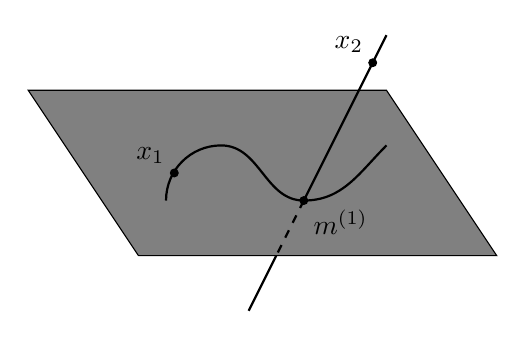
\begin{tikzpicture}[scale=0.7]
  \draw [fill=gray] (-.5,-1) -- (6,-1) -- (4,2) -- (-2.5,2) -- (-.5,-1);
  \draw [thick] (0,0) to [out=90,in=180] (1,1) to [out=0,in=180] (2.5,0) to [out=0,in=-135] (4,1);
  \draw [thick] (2.5,0) to (4,3);
  \draw [thick,dashed] (2.5,0) to (2,-1);
  \draw [thick] (2,-1) -- (1.5,-2);
  \draw [fill] (3.75,2.5) circle [radius=2pt] node[above left]{$x_2$};
  \draw [fill] (.15,.5) circle [radius=2pt] node[above left]{$x_1$};
  \draw [fill] (2.5,0.0) circle [radius=2pt] node[below right]{$m^{(1)}$};
 \end{tikzpicture}
\end{center}
and the invariants which contribute take the form
\begin{equation*} \bigg\langle \dfrac{i^*\eta_i}{z-\psi_1},\rho^h\bigg\rangle_{0,2,\beta^{(0)}}^Y \bigg\langle \rho_h, \mathbbm 1_{X}\bigg\rangle_{0,(m^{(1)},0),\beta^{(1)}}^{X|Y} \end{equation*}
for $i = 1, \ldots, k$ and $h = 1, \ldots, l$. By computing dimensions, we find
\begin{align*}
0\leq \codim \rho^h &= \dim Y-\codim \rho_h \\
&= \dim Y-\vdim \Q{0}{(m^{(1)},0)}{X|Y}{\beta^{(1)}} \\
&= \dim Y-(\dim X-3-K_{X}\cdot \beta^{(1)}+2-m^{(1)})\\
&= K_Y \cdot \beta^{(1)} - Y \cdot \beta^{(1)}+m^{(1)} \\
&\leq 0
\end{align*}
where the final equality follows from adjunction and the final inequality holds because $-K_Y$ is nef and $m^{(1)}\leq Y \cdot \beta_1$. This shows that the only non-trivial contributions come from curve classes $\beta^{(1)}$ such that $K_Y \cdot \beta^{(1)}=0$, and that in this case the order of tangency must be maximal, i.e. $m^{(1)}=Y \cdot \beta^{(1)}$. Furthermore we must have $\codim \rho^h = 0$ and so $\rho^h = \rho^1 = \mathbbm{1}_Y$ which implies $\rho_h = \rho_1 = \pt_Y$. Finally since $m^{(1)}=Y \cdot \beta^{(1)}$ we have
\begin{equation*} m = Y \cdot \beta^{(0)}+m^{(1)}=Y \cdot (\beta^{(0)} + \beta^{(1)}) = Y \cdot \beta \end{equation*}
and so again this piece only contrbutes to $T_{0,(Y\cdot\beta)}^{X|Y}(z,\beta)$, and the contribution is:
\begin{equation*} \sum_{i = 1}^{k} \bigg\langle \dfrac{i^*\eta_i}{z-\psi_1}, \mathbbm{1}_Y \bigg\rangle_{0,2,\beta^{(0)}}^Y \bigg\langle \pt_Y, \mathbbm{1}_X \bigg\rangle_{0,(Y \cdot \beta^{(1)},0),\beta^{(1)}}^{X|Y}\eta^i\end{equation*}
Finally, we must examine the terms of $T_{0,(m)}^{X|Y}(z,\beta)$ coming from:
\begin{equation*}\ev_{1*}(m\virt{\Q{0}{(m,0)}{X|Y}{\beta}})\end{equation*} 
Notice that we only have insertions from $i^*\HH^*(X) \subseteq \HH^*(Y)$ since $\ev_1$ is viewed as mapping to $X$. On the other hand
\begin{align*} \vdim \Q{0}{(m,0)}{X|Y}{\beta} & = \dim X-3 -K_X \cdot \beta +2-m & \\
& = \dim X - 1 -K_Y \cdot \beta + Y \cdot \beta - m \ \ & \text{by adjunction} \\
& \geq \dim X - 1 + Y\cdot\beta - m \ \ & \text{since $-K_Y$ is nef} \\
& \geq \dim X - 1 \ \ & \text{since $m \leq Y \cdot \beta$} \end{align*}
where in the second line we have applied the projection formula to $i$, and thus have implicity used Assumption (2), discussed in \S \ref{Subsection setup}; namely that every curve class on $X$ comes from a class on $Y$.

Consequently the only insertions that can appear are those of dimension $0$ and $1$. However, the restriction of the $0$-dimensional class $\eta_0 = \pt_X$ to $Y$ vanishes, as do the restrictions of all $1$-dimensional classes except for $\eta_1$ (by the definition of the dual basis, since $\eta^1 = Y$). Thus the only insertion is $i^*\eta_1$, and since this has dimension $1$ all the inequalities above must actually be equalities. This means that $-K_Y \cdot \beta = 0$ and $m = Y \cdot \beta$.

Once again, we see that there is only a contribution to $T_{0,(Y\cdot\beta)}^{X|Y}(z,\beta)$; this contribtion is:
\begin{equation*} m \left\langle \dfrac{i^* \eta_1}{z-\psi_1} , \mathbbm{1}_Y \right\rangle_{0,(Y \cdot \beta,0),\beta}^{X|Y} \eta^1 \end{equation*}

We have thus calculated $T_{0,(m)}^{X|Y}(z,\beta)$ for all $m$. We can thus write equation \eqref{eqn:G} as [UNDER CONSTRUCTION]




\begin{comment}
\begin{align*}
\prod_{j=0}^{Y\cdot\beta}(Y+jz) S_0^X(z,\beta) = T_{(Y\cdot\beta)}^{X|Y}(z,\beta) & = \sum_{i=1,\ldots,k;j\geq 0}z^{j+1}\eta^i\langle \rho_i\psi_1^j,\mathbbm 1_{Y}\rangle_{\Q{0}{2}{Y}{\beta}} \\
 &+\sum_{\substack{0<\beta^{(0)}<\beta \\ \beta^{(0)}+\beta^{(1)}=\beta}}z^{j+1}\eta^i\langle \rho_i\psi_1^j,\mathbbm 1_{Y}\rangle_{\Q{0}{2}{Y}{\beta^{(0)}}}(Y\cdot\beta^{(1)})\langle [pt_Y],\mathbbm 1_{X}\rangle_{\Q{0}{(Y\cdot\beta^{(1)},0)}{X|Y}{\beta^{(1)}}}\\
 &+\eta^1(Y\cdot\beta)\langle [pt_Y],\mathbbm 1_{X}\rangle_{\Q{0}{(Y\cdot\beta,0)}{X|Y}{\beta}}
\end{align*}
\end{comment}
if $\beta$ is such that $K_Y\cdot\beta=0$ (which implies $K_Y\cdot\beta^{(1)}=0$ as well, for every effective decomposition $\beta=\beta^{(0)}+\beta^{(1)}$, due to the semi-positivity assumption on $Y$); while, if $K_Y\cdot\beta<0$, it simply reduces to
\[
 \prod_{j=0}^{Y\cdot\beta}(Y+jz) S_0^X(z,\beta)= \sum_{i=1,\ldots,k;j\geq 0}z^{j+1}\eta^i\langle \rho_i\psi_1^j,\mathbbm 1_{Y}\rangle_{\Q{0}{2}{Y}{\beta}} = i_*S_0^Y(z,\beta).
\]


The proof of the first claim is now evident. We are left with evaluating $P(q)$.

In order to do that, we use again Gathmann's algorithm, this time in the opposite direction, to go all the way back to $X$; so it starts:
\[
 [\Q{0}{(Y \cdot \beta,0)}{X|Y}{\beta}]^\text{vir}=(Y+(Y\cdot\beta-1)\psi_1)[\Q{0}{(Y\cdot\beta-1,0)}{X|Y}{\beta}]^\text{vir}-[D_{Y\cdot\beta}^{\mathcal Q}(X|Y,\beta)]^\text{vir}
\]
When looking at the boundary, the invariants that come into play are of the form
\[
 \langle [pt_Y],\rho^h\rangle_{\Q{0}{2}{Y}{\beta^{(0)}}}\langle \rho_h,\mathbbm 1_{X}\rangle_{\Q{0}{(Y\cdot(\beta-\beta^{(0)})-1,0)}{X|Y}{\beta-\beta^{(0)}}}
\]
but notice that they must vanish by dimensional reasons, since
\[
 \codim(\rho^h)=\dim Y-3+2-K_Y\cdot\beta^{(0)}-\dim Y=-1.
\]
So
\begin{align*}
 & (Y\cdot\beta)\langle [pt_Y],\mathbbm 1_{X}\rangle_{\Q{0}{(Y\cdot\beta,0)}{X|Y}{\beta}} = \\
 & = (Y\cdot\beta)\int_{[\Q{0}{2}{X}{\beta}]^{\text{vir}}}\ev_1^*(\eta_1)\prod_{j=0}^{Y\cdot\beta-1}(\ev_1^*Y+j\psi_1) = \\
 & = (Y\cdot\beta)!\langle[pt_X]\psi_1^{Y\cdot\beta-1},\mathbbm 1_X\rangle_{\Q{0}{2}{X}{\beta}}.
\end{align*}
the second equality because $Y\cdot\eta_1=[pt_X]$ and $Y^2.\eta_1=0$.
\end{proof}

\begin{cor}
 If $Y$ is itself Fano, then there is no correction term
 \[
  \sum_{\beta\geq 0} q^\beta\prod_{j=0}^{Y\cdot\beta}(Y+jz)S_0^X(z,\beta) = i_*S_0^Y(z,q)
 \]
\end{cor}

\begin{cor}
 Let $Y_5$ be the quintic three-fold in $\PP^4$. Then
 \[
  i_*S_0^{Y_5}(z,q)=\frac{I_{\text{small}}^{Y_5}(z,q)}{P^{Y_5}(q)},
 \]
where
\[
 I_{\text{small}}^{Y_5}(z,q)=5H+\sum_{d>0}\frac{\prod_{j=0}^{5d}(H+jz)}{\prod_{j=0}^{d}(H+jz)^5}q^d
\]
and
\[
 P^{Y_5}(q)=1+\sum_{d>0}\frac{(5d)!}{(d!)^5}q^d.
\]
\end{cor}

\begin{remark}
 This formula (and, more generally, formulae for concavex bundles over products of projective spaces) was already obtained in \cite[Theorem 1]{CZ-mirror} via equivariant localisation.
\end{remark}

\subsection{Comparison with the work of Ciocan-Fontanine and Kim}

We would like to compare our formula to \cite[Corollary 5.5.1]{CF-K-wallcrossing}.

In \cite[Section 5]{CF-K-wallcrossing} they introduce (in the more general context of $\epsilon$-stable quasimaps to GIT quotients)
\begin{itemize}
 \item the $J^{\epsilon}$-function:
 \[
  J^\epsilon({\bf t}, z)=\sum_{k\geq 0,\beta\geq 0}q^\beta(\ev_\bullet)_*\left(\frac{\prod_{i=1}^k ev_i^*({\bf t})}{k!}\cap\operatorname{Res}_{F_0}[\QGe{0}{k}{Y}{\beta}]^{\text{vir}}\right)
 \]
\item the $S^\epsilon$-operator
\[
 S^\epsilon(z)(\gamma)=\sum_{m\ge 0,\beta\ge 0}\frac{q^\beta}{m!} 
(ev_1)_*\left(\frac{[\Qe{0}{2+m}{Y}{\beta}]^{\text{vir}}}{z-\psi}ev_2^*(\gamma)\prod_{j=3}^{2+m}ev_j^*({\bf t})\right)
\]
\item the $P^\epsilon$-series
\[
 P^\epsilon({\bf t}, z)=\sum_h\rho^h\sum_{m\geq 0,\beta\geq 0} \frac{q^\beta }{m!}
[\QGe{0}{1+m}{Y}{\beta}]\cap \ev_1^*(\rho_h p_\infty)
\]
where $p_\infty\in H^*_{\Gm}(\PP^1)$ is defined via its restrictions to the $\Gm$-fixed points: $p_{\infty|0}=0,p_{\infty|\infty}=-z$.
\end{itemize}
They prove by localisation that \cite[Theorem 5.4.1]{CF-K-wallcrossing}
\[
 J^\epsilon(z)=S^\epsilon(z)(P^\epsilon).
\]
Furthermore, they prove that, restricting to ${\bf t}=0$ and semi-positive targets, the only class that matches non-trivially with $P^\epsilon_{|{\bf t}=0}$ is $[pt_Y]$, and the above formula takes the simpler form of a product \cite[Corollary 5.5.1]{CF-K-wallcrossing}
\[
 \frac{J^\epsilon |_{{\bf t}=0}}{\langle [pt_Y],  P^\epsilon|_{{\bf t}=0}\rangle}=\mathbbm 1_Y+\sum_h\rho^h(\sum_{\beta\neq 0}q^\beta\langle\frac{\rho_h}{z-\psi},\mathbbm 1_Y\rangle_{0,2,\beta}^\epsilon).
\]
Notice that the restriction of $S^\epsilon(z)(\mathbbm 1_Y)$ to ${\bf t}=0$ that appears on the RHS of this formula coincides with what we have called $S^Y_0(z,q)$ above.

They also observe that, if we write the $\frac{1}{z}$-expansion of $J^{\epsilon}_{{\bf t}=0}$ as
\[
 J^{\epsilon}_{{\bf t}=0}=J^{\epsilon}_{0}(q)\mathbbm 1_Y+O(\frac{1}{z})
\]
then $\langle [pt_Y],  P^\epsilon|_{{\bf t}=0}\rangle=J^{\epsilon}_{0}(q)$.

Let us look more closely at $J^{\epsilon}_{{\bf t}=0}=\sum_{\beta\geq 0}q^\beta(\ev_\bullet)_*\left(\operatorname{Res}_{F_0}[\QGe{0}{0}{Y}{\beta}]^{\text{vir}}\right)$. Recall that in our context $Y\subseteq X$ is a very ample hypersurface and $X$ is toric Fano. Furthermore, set $\epsilon=0^+$. We have the following diagram:

\begin{center}
 \begin{tikzcd}
  \QG{0}{0}{Y}{\beta}\ar[d,hook,"\iota"]\ar[dr,phantom,"\Box"] & F_0^Y\ar[d]\ar[l,hook]\ar[r,"\ev_{\bullet}"] & Y\ar[d,hook,"i"] \\
  \QG{0}{0}{X}{\beta} & F_0^X\ar[l,hook]\ar[r,"\ev_{\bullet}"] & X
 \end{tikzcd}
\end{center}

\begin{itemize}[leftmargin=*]
 \item By a slight generalisation of \cite[Propositions 6.2.2 and 6.2.3]{CFKM}, $\iota_*[\QG{0}{0}{Y}{\beta}]^{\text{vir}}=e(\pi_* E^Y_{0,0,\beta}(z))\cap[\QG{0}{0}{X}{\beta}]^{\text{vir}}$ as $\Gm$-equivariant classes, where $\pi$ is the universal curve on $\QG{0}{0}{X}{\beta}$ and $E^Y_{0,0,\beta}(z)$ is the equivariant line bundle on it associated to $\mathcal O_X(Y)$. This is analagous to the bundle $L_Y$ used in the definition of relative quasimaps (see \S \ref{Subsection relative stable quasimaps}).
\item Since the fibers of $\pi$ are irreducible (by the stability condition and the fact that there are no markings, there can only be the parametrised component), the following splitting holds:
 \[
  e(\pi_* E^Y_{0,0,\beta}(z))=\prod_{j=0}^{Y\cdot\beta} c_1(\sigma_0^* E^Y_{0,0,\beta}(z)\otimes \omega_{\pi}^{\otimes j})
 \]
coming from evaluating at (the $j$-th order infinitesimal thickening of) the zero section $\sigma_0$ and the jet bundles exact sequence:
\begin{center}
 \begin{tikzcd}
  0\ar[r] & \pi_* (E^Y_{0,0,\beta}(-j\sigma_0))\ar[r] & \pi_* E^Y_{0,0,\beta}\ar[r] & \sigma_0^*\operatorname{P}^{j-1}(E^Y_{0,0,\beta}) \ar[r] & 0 \\
  0\ar[r] & \Omega_\pi^{\otimes j}\otimes E^Y_{0,0,\beta}\ar[r] & \operatorname{P}^{j}(E^Y_{0,0,\beta}) \ar[r] & \operatorname{P}^{j-1}(E^Y_{0,0,\beta}) \ar[r] & 0
 \end{tikzcd}
\end{center}
which, restricting to $F_0^X$, gives:
\[
 \iota_*[F_0^Y]^{\text{vir}}=\prod_{j=0}^{Y\cdot\beta}(Y+iz)[F_0^X]^{\text{vir}}.
\]
 \item The small $J^{0^+}$-function for toric varieties has been evaluated by Givental \cite{Givental-equivariantGW}\cite[Definition 7.2.8]{CF-K}:
 \[
  (\ev_{\bullet})_*\frac{[F_0^X]^{\text{vir}}}{e(N_{F_0/\QG{0}{0}{X}{\beta}})}=\prod_{\rho\in\Sigma_X(1)}\frac{\prod_{j=-\infty}^0(D_{\rho}+jz)}{\prod_{j=-\infty}^{\int_{\beta}D_{\rho}}(D_\rho+jz)}=\frac{\prod_{\substack{\rho\in\Sigma_X(1)\colon D_\rho.\beta\leq 0 \\ j=\int_{\beta}D_\rho,\ldots,0}}(D_{\rho}+jz)}{\prod_{\substack{\rho\in\Sigma_X(1)\colon D_\rho.\beta> 0 \\ j=1,\ldots,\int_{\beta}D_\rho}}(D_{\rho}+jz)}
 \]
So, using $\sum_{\rho\in\Sigma_X(1)} D_{\rho}=-K_X$ and $(Y+K_X).\beta=0$, we see that
\[
 J^Y_0(q)=\sum_{\beta\geq 0}q^\beta(Y\cdot\beta)!\frac{\prod_{\rho\in\Sigma_X(1)\colon D_\rho.\beta< 0}(-1)^{-D_{\rho}.\beta}(-D_{\rho}.\beta)!}{\prod_{\rho\in\Sigma_X(1)\colon D_\rho.\beta> 0}(D_{\rho}.\beta)!}
\]
\item Since $X$ is Fano, $J^X_{|{\bf t}=0}=S^X_{|{\bf t}=0}(\mathbbm 1_X)$.
\item The coefficient $\langle[pt_X]\psi_1^{Y\cdot\beta-1},\mathbbm 1_X\rangle_{\Q{0}{2}{X}{\beta}}$ that appears in our $P$-series (multiplied by $(Y\cdot\beta)!$), can be deduced from the expansion of $S^X_{|{\bf t}=0}(\mathbbm 1_X)$ given above, and it turns out to be
\[
 \langle [pt_X],S^X_{|{\bf t}=0}(\mathbbm 1_X)\rangle[z^{Y\cdot\beta}]=\frac{\prod_{\rho\in\Sigma_X(1)\colon D_\rho.\beta< 0}(-1)^{-D_{\rho}.\beta}(-D_{\rho}.\beta)!}{\prod_{\rho\in\Sigma_X(1)\colon D_\rho.\beta> 0}(D_{\rho}.\beta)!}.
\]

\end{itemize}

So we may conclude that the $i_*$ of \cite[Corollary 5.5.1]{CF-K-wallcrossing} coincides with our Equation \ref{eqn:mirror}.

\appendix

In this appendix we collect several foundational results in quasimap theory, including:
\begin{enumerate}
\item \ilemph{Functoriality} (\S \ref{Functoriality of Quasimap Spaces Section}): given a morphism $f\colon Y\to X$ we describe the induced map:
\begin{equation*} \om{Q}(f)\colon\Q{g}{n}{Y}{\beta}\to\Q{g}{n}{X}{f_*\beta} \end{equation*}
We also discuss (\S \ref{section:rel_pot_for_qm_functoriality}) when $\om{Q}(f)$ admits a compatible perfect obstruction theory.
\item \ilemph{Splitting axiom} (\S \ref{Subsection splitting}): this gives an equality between two natural virtual classes on boundary strata (i.e. loci where the underlying curve is reducible of a prescribed type).
\item \ilemph{Comparison with the GIT construction} (\S \ref{Section comparison with GIT construction}): we show that for a (not necessarily toric) hypersurface $Y \hookrightarrow X$, our definition of $\om{Q}(Y)$ as a substack of $\om{Q}(X)$ coincides with the definition of $\om{Q}(Y)$ given by the description of $Y$ as a GIT quotient (see \cite{CFKM}).
\end{enumerate}

\subsection{Functoriality} \label{Functoriality of Quasimap Spaces Section}

In the case of stable maps, a morphism $f : Y \to X$ induces a morphism between the corresponding moduli spaces
\begin{equation*}\om{M}(f) : \M{g}{n}{Y}{\beta} \rightarrow \M{g}{n}{X}{f_* \beta} \end{equation*}
given by post-composition with $f$ (in general we may have to stabilise the source curve). Because of this, we may say that the construction of the moduli space of stable maps is \ilemph{functorial}.

It is natural to ask whether the same holds for the moduli space of quasimaps, i.e. whether we have a morphism:
\begin{equation*} \om{Q}(f) : \Q{g}{n}{Y}{\beta} \to \Q{g}{n}{X}{f_* \beta} \end{equation*}
Since here the objects of the moduli space are not maps, we cannot simply compose with $f$. Nevertheless, our definition should be equivalent to composing with $f$ when applied to a quasimap without any basepoints. In \cite[Section 3.1]{CF-K-wallcrossing} a definition (in the GIT context) is given when $f$ is an embedding into a projective space; we shall discuss the general situation of a morphism between toric varieties $f\colon Y\to X$.

Our approach uses the language of $\Sigma$--collections introduced by D. A. Cox. This approach is natural insofar as a quasimap is a generalisation of a $\Sigma$--collection. We will refer extensively to \cite{CoxRing} and \cite{CoxFunctor}.

Let $X$ and $Y$ be smooth and proper toric varieties with fans $\Sigma_X \subseteq N_X$ and $\Sigma_Y \subseteq N_Y$. Suppose we are given $f : Y \to X$ (which we do not assume to be a toric morphism). By \cite[Theorem 1.1]{CoxFunctor} the data of such a map is equivalent to a $\Sigma_X$--collection on $Y$:
\begin{equation*} ( (L_\rho, u_\rho)_{\rho \in \Sigma_X(1)}, (\varphi_{m_x})_{m_x \in M_X} ) \end{equation*}
In addition, \cite{CoxRing} allows us to describe line bundles on $Y$ and their global sections in terms of the homogeneous coordinates $(z_\tau)_{\tau \in \Sigma_Y(1)}$. All of these observations are combined into the following theorem, which is so useful that we will state it here in its entirety:

\begin{thm} \cite[Theorem 3.2]{CoxFunctor} \label{CoxTheorem} The data of a morphism $f:Y \to X$ is the same as the data of homogeneous polynomials
\begin{equation*} P_\rho \in S^Y_{\beta_\rho} \end{equation*}
for $\rho = f^* \OO_X(D_\rho) \in \Sigma_X(1)$, where $\beta_\rho \in \Pic Y$ and $S^Y_{\beta_\rho}$ is the corresponding graded piece of the Cox ring:
\begin{equation*}S^Y = \CC[z_\tau : \tau \in \Sigma_Y(1)]\end{equation*}
This data is required to satisfy the following two conditions:
\begin{enumerate}
\item $\sum_{\rho \in \Sigma_X(1)} \beta_\rho \otimes n_\rho = 0$ in $\Pic Y \otimes N_X$, where $n_\rho$ is the principal generator of the ray $\rho$.
\item $(P_\rho(z_\tau)) \notin Z(\Sigma_X) \subseteq \Aaff^{\Sigma_X(1)}$ whenever $(z_\tau) \notin Z(\Sigma_Y) \subseteq \Aaff^{\Sigma_Y(1)}$.
\end{enumerate}
Furthermore, two such sets of data $(P_\rho)$ and $(P^\prime_\rho)$ correspond to the same morphism if and only if there exists a $\lambda \in \Hom_\Z(\Pic X, \Gm)$ such that
\begin{equation*} \lambda(D_\rho) \cdot P_\rho = P^\prime_\rho \end{equation*}
for all $\rho \in \Sigma_X(1)$. Finally, if we define $\tilde{f}(z_\tau) = (P_\rho(z_\tau))$ then this defines a lift of $f$ to the prequotients:
\bcd
\Aaff^{\Sigma_Y(1)} \setminus Z(\Sigma_Y) \ar[r, "\tilde{f}"] \ar[d, "q_Y"] & \Aaff^{\Sigma_X(1)} \setminus Z(\Sigma_X) \ar[d,"q_X"] \\
Y \ar[r, "f"] & X
\ecd
\end{thm}
\begin{aside} Throughout this section we will stick to the notation established above; in particular we will use $\rho$ to denote a ray in $\Sigma_X(1)$ and $\tau$ to denote a ray in $\Sigma_Y(1)$. \end{aside}

Recall our goal: given a map $f \colon Y \to X$ we wish to define a ``push-forward'' map:
\begin{equation*} \om{Q}(f) : \Q{g}{n}{Y}{\beta} \to \Q{g}{n}{X}{f_*\beta} \end{equation*}
Consider therefore a quasimap
\begin{equation*} ((C,x_1,\ldots,x_n), (L_\tau, u_\tau)_{\tau \in \Sigma_Y(1)}, (\varphi_{m_Y})_{m_Y \in M_Y}) \in \Q{g}{n}{Y}{\beta} \end{equation*}
over an arbitrary base. Pick data $(P_\rho)_{\rho \in \Sigma_X(1)}$ corresponding to the map $f$, as in the theorem above; we will later see that our construction does not depend on this choice.

The idea of the construction is as follows. Locally around a point $x~\in~U_x \subseteq C$ we can trivialise the $L_\tau$ to obtain a morphism to the prequotient
\begin{equation*} (u_\tau)_\tau \colon U_x \to \Aaff^{\Sigma_Y(1)} \end{equation*}
which lifts the induced rational map to $Y$. On the other hand the data of $(P_\rho)_\rho$ gives a lifting of $f\colon Y\to X$ to a morphism between the prequotients
\begin{equation*}(P_\rho)_\rho \colon \Aaff^{\Sigma_Y(1)} \to \Aaff^{\Sigma_X(1)}\end{equation*}
and so the composed map to the prequotient of $X$ is given by:
\begin{equation*} (P_\rho((u_\tau)_\tau))_\rho : U_x \to \Aaff^{\Sigma_X(1)} \end{equation*}
In order to define the pushed-forward quasimap, we thus need to make sense of $P_\rho((u_\tau)_\tau)$ as a section of a certain line bundle $\tilde{L}_\rho$ on the curve.

We now make this precise. The first issue to address is the stabilisation of the source curve. The procedure is the same as in the case of stable maps: if $C_0 \subseteq C$ is a rational component with $2$ special points (hence with curve class $\beta_0 > 0$) and such that $f_* \beta_0 = 0$, then $C_0$ should be contracted when we pass to $X$. The possibilities are:

\begin{center}
\begin{tikzpicture}[scale=0.5]
\draw (0,0) -- (1,3) node[above]{$\beta_1$} (0,1) -- (1,-2) node[below]{$\beta_0$};
\draw[fill=black] (0.66,-1) circle[radius=2pt];
\draw[->,decorate,decoration=snake] (2,0.5) -- (4,0.5);
\draw (5,0) -- (6,3) node[above]{$f_*\beta_1$};
\draw[fill=black] (5.16,.5) circle[radius=2pt];

\draw (10.33,-1.5) -- node[right]{$\beta_0$} (10.33,2.5) (10,1) -- (11,4) node[above]{$\beta_1$} (10,0) -- (11,-3) node[below]{$\beta_2$};
\draw[->,decorate,decoration=snake] (12,0.5) -- (14,0.5);
\draw (15,0) -- (16,3) node[above]{$f_*\beta_1$} (15,1) -- (16,-2) node[below]{$f_*\beta_2$};
\end{tikzpicture}
\end{center}
To perform the contraction we need to construct a line bundle on $C$ which is trivial on the components which we wish to contract and ample (relative to the base) on all the other components.

Fix a polarisation $\OO_X(1)$ on $X$ and express $f^*\OO_X(1)$ in terms of the toric divisors of $Y$:
\begin{equation*} f^*\OO_X(1) = \bigotimes_\tau \OO_Y(D_\tau)^{\otimes c_\tau} \end{equation*}
Then the line bundle
\begin{equation*} \omega_{\pi}(x_1+\ldots+x_n)\otimes \bigotimes_\tau L_\tau^{\otimes a_\tau} \end{equation*}
gives the required contraction by taking relative Proj. We thus obtain a curve $\tilde{C}$ and a morphism $\phi : C \to \tilde{C}$ which contracts the unstable components.

Recall that for $\rho \in \Sigma_X(1)$, $P_\rho$ is a polynomial in the $z_\tau$. We can thus write it as
\begin{equation} \label{Prho} P_\rho(z_\tau) = \sum_{\underline{a}} P_\rho^{\underline{a}}(z_\tau) = \sum_{\underline{a}} \mu_{\underline{a}} \prod_{\tau} z_{\tau}^{a_{\tau}} \end{equation}
where the sum is over a finite number of multindices $\underline{a} = (a_\tau) \in \N^{\Sigma_Y(1)}$ and the $\mu_{\underline{a}}$ are nonzero scalars. Observe that, for each $\underline{a}$, the line bundle $\otimes_\tau  L_\tau^{\otimes a_\tau}$ on $C$ is trivial on the components contracted by $\phi$ (which are always rational). Hence, by cohomology and base-change, it descends to a line bundle on $\tilde{C}$:
\begin{equation*} \tilde{L}_\rho^{\underline{a}} :=\phi_* \bigotimes_\tau L_\tau^{\otimes a_\tau} \end{equation*}
We may then take the following section of $\tilde{L}_\rho^{\underline{a}}$:
\begin{equation*} \tilde{u}_\rho^{\underline{a}} = P_\rho^{\underline{a}}(u_\tau) := \mu_{\underline{a}} \prod_\tau u_\tau^{a_\tau}; \end{equation*}
A priori this is really a section of $\otimes_\tau L_\tau^{\otimes a_\tau}$ on $C$; but since it is constant on the components contracted by $\phi$, it descends to a section of $\tilde{L}_\rho^{\underline{a}}$ on $\tilde{C}$.

Thus, each of the terms $P_\rho^{\underline{a}}$ of $P_\rho$ defines a section $\tilde{u}_\rho^{\underline{a}}$ of a line bundle $\tilde{L}_\rho^{\underline{a}}$ on $\tilde{C}$. What we want, however is a single section $\tilde{u}_\rho$ of a single line bundle $\tilde{L}_\rho$. This is where the isomorphisms $\varphi_{m_Y}$ come in.

Recall that we have a short exact sequence:
\begin{equation} \label{Pic short exact sequence for Y} 0 \longrightarrow M_Y \overset{\theta}{\longrightarrow} \Z^{\Sigma_Y(1)} \longrightarrow \Pic Y \longrightarrow 0 \end{equation}
Let $\underline{a}$ and $\underline{b}$ be multindices appearing in the sum \eqref{Prho} above. By the homogeneity of $P_\rho$ we have
\begin{equation*} \sum_\tau a_\tau [D_\tau] = \beta_\rho = \sum_\tau b_\tau [D_\tau] \end{equation*}
which is precisely the statement that in the above sequence $\underline{a}$ and $\underline{b}$ map to the same element of $\Pic Y$ (namely $\beta_\rho$). Hence there exists a unique $m_Y \in M_Y$ such that:
\begin{equation*} \theta(m_Y) = \underline{a} - \underline{b} \end{equation*}
Now, the isomorphism $\varphi_{m_Y}$ (contained in the data of our original quasimap) is a map:
\begin{equation*} \varphi_{m_Y} : \bigotimes_\tau L_\tau^{\otimes \langle m_Y, n_\tau \rangle} \cong \OO_{C} \end{equation*}
By definition, $\theta(m_Y) = (\langle m_Y,n_\tau \rangle)_{\tau \in \Sigma_Y(1)}$. But also $\theta(m_Y) = (a_\tau - b_\tau)_{\tau \in \Sigma_Y(1)}$. Hence we have:
\begin{equation*} \varphi_{m_Y} : \bigotimes_\tau L_\tau^{\otimes a_\tau} \cong \bigotimes_\tau L_\tau^{\otimes b_\tau} \end{equation*}
This descends to give canonical isomorphisms
\begin{equation*} \tilde{L}_\rho^{\underline{a}} \cong \tilde{L}_\rho^{\underline{b}} \end{equation*}
for all $\underline{a}$ and $\underline{b}$. Let us choose one such $\underline{a}$ (it doesn't matter which); call it $\underline{a}^\rho$. We define:
\begin{equation*} \tilde{L}_\rho := \tilde{L}_\rho^{\underline{a}^\rho} \end{equation*}
Then for all $\underline{b}$ we can use the above isomorphisms to view $\tilde{u}_\rho^{\underline{b}}$ as a section of $\tilde{L}_\rho$. Summing all of these together we thus obtain a section $\tilde{u}_\rho$ of $\tilde{L}_\rho$, which we can write (with abuse of notation) as:
\begin{equation*} \tilde{u}_\rho = \sum_{\underline{a}} \mu_{\underline{a}} \prod_\tau u_\tau^{a_\tau} \end{equation*}
Note that if we had made a different choice of $\underline{a}^\rho$ above the result would have been isomorphic.

Thus far we have constructed line bundles and sections $(\tilde{L}_\rho, \tilde{u}_\rho)_{\rho \in \Sigma_X(1)}$ on $\overline{\mathcal C}$. It remains to define the isomorphisms
\begin{equation*} \tilde{\varphi}_{m_X} : \otimes_\rho \tilde{L}_\rho^{\otimes \langle m_X, n_\rho \rangle} \cong \OO_{\tilde{C}} \end{equation*}
for all $m_X \in M_X$. The left hand side is:
\begin{align*} \otimes_\rho \tilde{L}_\rho^{\otimes \langle m_X, n_\rho \rangle} & = \otimes_\rho \left( \phi_* \otimes_\tau L_\tau^{\otimes a_\tau^\rho} \right)^{\otimes \langle m_X, n_\rho \rangle} = \phi_* \otimes_\tau L_\tau^{\otimes \left( \sum_{\rho} a_\tau^\rho  \langle m_X, n_\rho \rangle \right)} \end{align*}
Now, for $m_Y \in M_Y$ we have isomorphisms $\varphi_{m_Y} : \otimes_\tau L_\tau^{\otimes \langle m_Y, n_\tau \rangle} \cong \OO_{C}$. In order to construct $\tilde{\varphi}_{m_X}$ it is therefore tempting to look for an $m_Y$ such that
\begin{equation*} \langle m_Y, n_\tau \rangle = \sum_\rho a_\tau^\rho \langle m_X, n_\rho \rangle \end{equation*}
for all $\tau \in \Sigma_Y(1)$ (we will then set $\tilde{\varphi}_{m_X} = \varphi_{m_Y}$). Consider therefore the short exact sequence \eqref{Pic short exact sequence for Y}. Recall that $\theta(m_Y) = (\langle m_Y, n_\tau \rangle)_{\tau \in \Sigma_Y(1)}$. Hence we need to show that
\begin{equation*} \left( \sum_\rho a_\tau^\rho \langle m_X, n_\rho \rangle \right)_{\tau \in \Sigma_Y(1)} \end{equation*}
belongs to the image of $\theta$, i.e. that it belongs to the kernel of the second map (notice that $m_Y$ is then unique because $\theta$ is injective). This is equivalent to saying that
\begin{equation*} \sum_\tau \sum_\rho a_\tau^\rho \langle m_X, n_\rho \rangle [D_\tau] = 0 \in \Pic Y \end{equation*}
Now, we have
\begin{equation*} \sum_\tau a_\tau^\rho [D_\tau] = \beta_\rho \end{equation*}
so that the above sum becomes
\begin{equation*} \sum_\rho \langle m_X, n_\rho \rangle \beta_\rho = \left\langle m_X, \sum_\rho \beta_\rho \otimes n_\rho \right \rangle = \langle m_X, 0 \rangle = 0 \end{equation*}
where $\sum_\rho \beta_\rho \otimes n_\rho = 0$ by Condition (1) in Theorem \ref{CoxTheorem}. So there does indeed exist a (unique) $m_Y \in M_Y$ such that $\langle m_Y, n_\tau \rangle = \sum_\rho a_\tau^\rho \langle m_X, n_\rho \rangle$, so that we can set:
\begin{equation*} \tilde{\varphi}_{m_X} = \varphi_{m_Y} : \bigotimes_\rho \tilde{L}_\rho^{\otimes \langle m_X, n_\rho \rangle} \cong \OO_{\overline{\mathcal C}} \end{equation*}
Thus, we have produced a quasimap with target $X$ and class $f_*\beta$ on the base $\Q{g}{n}{Y}{\beta}$:
\begin{equation*} ((\tilde{C},\tilde{x_1},\ldots,\tilde{x_n}), (\tilde{L}_\rho, \tilde{u}_\rho)_{\rho \in \Sigma_X(1)}, (\tilde{\varphi}_{m_X})_{m_X \in M_X}) \end{equation*}
The proof that this construction does not depend on the choice of $(P_\rho)$ is straightforward and is left to the reader.

It remains to demonstrate that the quasimap thus constructed is nondegenerate and stable. Nondegeneracy follows immediately from Condition (2) in Theorem \ref{CoxTheorem}. Put differently: the original quasimap defined a rational map $C \dashrightarrow Y$, whereas the new quasimap defines a rational map which is simply the composition $C \dashrightarrow Y \to X$ (up to contracting unstable components). Therefore the set of basepoints is exactly the same.

Stability follows precisely from the construction of $\phi$: if we write the polarisation of $X$ as $\OO_X(1) = \bigotimes_\rho \OO(D_\rho)^{\otimes b_\rho}$ then 
\begin{equation*} \omega_{\tilde{\pi}}(\bar x_1+\ldots \bar x_n)\otimes\bigotimes_\rho \tilde{L}_\rho^{\otimes b_\rho} \end{equation*}
will be $\tilde\pi$-ample on $\tilde{C}$, since we have contracted all the components on which $f^*\OO_X(1)$ was trivial without introducing any rational tail.

To summarise, we have explained how to canonically associate, to any family of quasimaps with target $Y$, a family of quasimaps with target $X$. This completes the proof of the following:

\begin{thm} \label{functoriality proposition} Let $X$ and $Y$ be smooth proper toric varieties and $f : Y \to X$ a morphism. Then there exists a natural push-forward map:
\begin{equation*} \om{Q}(f) \colon \Q{g}{n}{Y}{\beta} \to \Q{g}{n}{X}{f_* \beta} \end{equation*}\end{thm}
 	
\begin{remark}
 Theorem \ref{CoxTheorem} tells us that we can lift any morphism between toric varieties to an equivariant morphism between the prequotients
\bcd
 \Aaff^{\Sigma_Y(1)} \setminus Z(\Sigma_Y) \ar[r, "\tilde{f}"] \ar[d, "q_Y"] & \Aaff^{\Sigma_X(1)} \setminus Z(\Sigma_X) \ar[d,"q_X"] \\
 Y \ar[r, "f"] & X
\ecd
where the torus homomorphism
\begin{equation*} G_Y=\Hom_{\mathbb Z}(\Pic(Y), \Gm)\to G_X=\Hom_{\mathbb Z}(\Pic(Y),\Gm) \end{equation*}
is induced in the obvious way by $f\colon Y\to X$. Now, thinking of quasimaps as maps to the quotient stack, functoriality is again clear by postcomposition with $\tilde{f}$ (notice that the preimage of the unstable locus of $X$ is the unstable locus of $Y$).
\end{remark}

Finally, let us describe how this push-forward morphism behaves when $f$ is a nonconstant map $\PP^r \to \PP^N$. Write $f$ in homogeneous coordinates as:
\begin{equation*} f[z_0, \ldots, z_r] = [f_0(z_0, \ldots, z_r), \ldots, f_N(z_0, \ldots, z_r)] \end{equation*}
where the $f_i$ are all homogeneous of degree $a>0$. Then given a quasimap with target $\PP^r$
\begin{equation*} (C, L, u_o, \ldots, u_r) \end{equation*}
the pushed-forward quasimap with target $\PP^N$ is:
\begin{equation*} (C, L^{\otimes a}, f_0(u_0, \ldots, u_r) , \ldots, f_N(u_0, \ldots, u_r)) \end{equation*}

\subsection{Relative obstruction theories for $\om{Q}(Y)\to\om{Q}(X)$}\label{section:rel_pot_for_qm_functoriality}
Assume now that $f\colon Y\to X$ is a morphism (between projective varieties) satisfying any of the following three equivalent conditions:
\begin{enumerate}
 \item $f$ is finite;
 \item for any ample line bundle $\OO_X(1)$ on $X$, $f^*\OO_X(1)$ is ample on $Y$;
 \item for every effective curve class $\beta\in \HH_2^+(Y)$, $f_*\beta\neq 0$.
\end{enumerate}
These conditions are in particular satisfied when $f$ is a closed embedding, which is the case of most interest to us.

Observe then that the induced morphism $$k=\om{Q}(f) \colon \Q{g}{n}{Y}{\beta} \to \Q{g}{n}{X}{f_* \beta}$$ commutes with the projections to $\mathfrak M_{g,n}$, i.e. there is no need to stabilise the underlying curve. We would like to have a pull-back morphism $k^!$ for the Chow groups. However, even in the easiest possible case when $f \colon Y \hookrightarrow X$ is a regular embedding, $k$ itself is not necessarily a regular embedding, and so the Gysin map in the sense of \cite{FUL} is not guaranteed to exist.

However, when $\Q{g}{n}{X}{f_* \beta}$ is unobstructed (for instance when $X=\PP^N$ and $g=0$ or $(g,n)=(1,0)$) there is a way around this. In \cite{Manolache-Pull} a generalisation of the Gysin map called the \ilemph{virtual pull-back} is defined for morphisms endowed with a relative perfect obstruction theory. Moreover, a sufficient condition is given \cite[Corollary 4.9]{Manolache-Pull} for this map to respect the virtual classes.

\begin{lem} \label{Exists relative POT} For a \emph{finite} morphism of smooth toric varieties $f\colon Y\to X$, there exists a relative obstruction theory $\EE_k$ for the morphism
\begin{equation*} k : \Q{g}{n}{Y}{\beta} \to \Q{g}{n}{X}{f_*\beta} \end{equation*}
which fits into a compatible triple with the standard obstruction theories for the quasimap spaces over $\MM_{g,n}$. Furthermore, $\EE_k$ is perfect \emph{if $\Q{g}{n}{X}{f_*\beta}$ is unobstructed}, so that:
\begin{equation*} k^!_{\operatorname{v}} [ \Q{g}{n}{X}{f_*\beta} ] = \virt{\Q{g}{n}{Y}{\beta}} \end{equation*} \end{lem}

\begin{proof} Note first that, since $k$ does not change the source curve of a quasimap, we indeed have a commuting triangle:
\bcd
\Q{g}{n}{Y}{\beta} \ar[rr,"k"] \ar[rd] & & \Q{g}{n}{X}{f_*\beta} \ar[ld] \\
& \MM_{g,n} & 
\ecd
We have perfect obstruction theories $\EE_{\om{Q}(Y)/\MM}$ and $\EE_{\om{Q}(X)/\MM}$ and we want to find a perfect obstruction theory $\EE_k$. Consider the diagram of universal curves
\bcd
\mathcal{C}_Y \ar[r,"\alpha"] \ar[d,"\pi"] \ar[rd,phantom,"\square" right] & \mathcal{C}_{X} \ar[d,"\rho"] \\
\Q{g}{n}{Y}{\beta} \ar[r,"k"] & \Q{g}{n}{X}{f_*\beta}
\ecd
which is cartesian because $k$ does not alter the source curve of any quasimap. We have sheaves $\mathcal{F}_Y$ and $\mathcal{F}_{X}$ on $\mathcal{C}_Y$ and $\mathcal{C}_{X}$ respectively such that:
\begin{align*} \EE_{\om{Q}(Y)/\MM}^\vee & = \R \pi_* \mathcal{F}_Y \\
\EE_{\om{Q}(X)/\MM}^\vee & = \R \rho_* \mathcal{F}_{X} \end{align*}
It follows (by flatness of $\rho$) that when we pull back the latter obstruction theory to $\om{Q}(Y)$ we obtain:
\begin{equation*} k^* \EE_{\om{Q}(X)/\MM}^\vee = \R \pi_* \alpha^* \mathcal{F}_{X} \end{equation*}
To construct a compatible triple, we require a morphism $k^* \EE_{\om{Q}(X)/\MM} \to \EE_{\om{Q}(Y)/\MM}$. Dually, it is therefore enough to construct a morphism of sheaves on $\mathcal{C}_Y$
\begin{equation*} \mathcal{F}_Y \to \alpha^* \mathcal{F}_{X} \end{equation*}
and then apply $\R \pi_*$. This is analogous to the morphism $f^* T_Y \to f^* T_{X}|_Y$ which is used in the stable maps setting. However the construction for quasimaps requires a little more ingenuity, because we do not have access to a universal map $f$.

The sheaf $\mathcal{F}_Y$ is defined on $\mathcal{C}_Y$ by the short exact sequence
\begin{equation*} 0 \to \OO_{\mathcal{C}_Y}^{\oplus r_Y} \to \oplus_{\tau} \mathcal{L}_\tau \to \mathcal{F}_Y \to 0 \end{equation*}
where $r_Y = \operatorname{rk} \Pic Y$ (implicitly we have chosen a basis for $\Pic Y$). Similarly $\mathcal{F}_{X}$ is defined on $\mathcal{C}_{X}$ by:
\begin{equation*} 0 \to \OO_{\mathcal{C}_{X}}^{\oplus r_X} \to \oplus_{\rho} \mathcal{L}_\rho \to \mathcal{F}_{X} \to 0 \end{equation*}
We will construct the map $\mathcal{F}_Y \to \alpha^* \mathcal{F}_{X}$ by first constructing a morphism:
\begin{equation*} \oplus_{\tau} \mathcal{L}_\tau \to \alpha^* (\oplus_{\rho} \mathcal{L}_\rho) \end{equation*}
Recall that $f\colon Y\to X$ is given by homogeneous polynomials
\begin{equation*} P_\rho \in S^Y_{\beta_\rho} \subset S^Y = k[z_\tau : \tau \in \Sigma_Y(1)] \end{equation*}
in the Cox ring of $Y$, where $\beta_{\rho}=f^*[D_\rho] \in \Pic Y$. For all monomials appearing in $P_\rho$, if we look at their exponents $(a_{\tau})_{\tau\in\Sigma_Y(1)}$, we have $\sum_{\tau\in\Sigma_Y(1)}a_\tau[D_\tau]=\beta_\rho$ by homogeneity; hence we can use the isomorphisms parametrised by $M_Y$ as in the proof of Proposition \ref{functoriality proposition} above in order to interpret the $(P_\rho)$ as a morphism
\begin{equation*} (P_\rho)_{\rho\in\Sigma_X(1)}\colon \bigoplus_{\tau} \mathcal{L}_{\tau} \to \bigoplus_{\rho} \bigotimes_{\tau} \mathcal{L}_\tau^{\otimes a_\tau^\rho} = \bigoplus_{\rho} \tilde{\mathcal{L}}_\rho = \alpha^* \left( \bigoplus_{\rho} \mathcal{L}_\rho \right) 
\end{equation*}
where the notation is as in the proof of functoriality in \S \ref{Functoriality of Quasimap Spaces Section}. Thus we have constructed a morphism $\oplus_{\tau} \mathcal{L}_\tau \to \alpha^* (\oplus_{\rho} \mathcal{L}_\rho)$.

On the other hand, $f\colon Y\to X$ induces a pullback map on line bundles $\Pic(X)\to\Pic(Y)$. Since we have implicitly chosen bases for these $\Z$-modules, this gives rise to a matrix, whose transpose we denote by:
\begin{equation*} Q\in \operatorname{Mat}_{r_X\times r_Y}(\Z) \end{equation*}
It is now clear by the functoriality construction that the left-hand square in the following diagram is commutative; hence it induces the (dashed) map of sheaves that we were after:
\begin{equation}\label{diagram:functoriality}
\begin{tikzcd}
0 \ar[r] & \OO_{C_Y}^{\oplus r_Y} \ar[r] \ar[d,"Q"] & \oplus_{\tau} \mathcal{L}_\tau \ar[r] \ar[d,"{(P_\rho)}"] & \mathcal{F}_Y \ar[d,dashed]\ar[r] & 0 \\
0 \ar[r] & \OO_{\mathcal{C}_{Y}}^{\oplus r_X} \ar[r] & \alpha^* \left(\oplus_{\rho} \mathcal{L}_\rho\right) \ar[r] & \alpha^* \mathcal{F}_{X} \ar[r] & 0
\end{tikzcd}
\end{equation}
Applying $\R \pi_*$ and dualising we obtain a morphism between the obstruction theories for the quasimap spaces, and we can complete this to obtain an exact triangle
\begin{equation*} k^* \EE_{\om{Q}(X)/\MM} \to \EE_{\om{Q}(Y)/\MM} \to \EE_k \xrightarrow{[1]}\end{equation*}
on $\om{Q}(Y)$. The axioms of a triangulated category then give a morphism of exact triangles:
\bcd
k^* \EE_{\om{Q}(X)/\MM} \ar[r] \ar[d] & \EE_{\om{Q}(Y)/\MM} \ar[r] \ar[d] & \EE_k  \ar[r,"{[1]}"] \ar[d] & \, \\
k^*\LL_{\om{Q}(X)/\MM} \ar[r] & \LL_{\om{Q}(Y)/\MM} \ar[r] & \LL_k \ar[r,"{[1]}"] & \,
\ecd
It follows from a simple diagram chase that $\EE_k \to \LL_k$ is a relative obstruction theory supported in $[-2,0]$. On the other hand, assuming that $\Q{g}{n}{X}{f_*\beta}$ is unobstructed, we may look at the long exact sequence in cohomology and find:
\begin{equation*} 0 \to \h^{-2}(\EE_k) \to \h^{-1}(k^* \EE_{\om{Q}(X)/\MM}) = 0\end{equation*}
Hence $\h^{-2}(\EE_k) = 0$ and so $\EE_k$ is perfect. \end{proof}

\begin{remark} The short exact sequence defining $\mathcal{F}_X$ should be thought of as the pull-back of the Euler sequence
\begin{equation*} 0 \to \OO_X^{\oplus r_X} \to \bigoplus_{\rho \in \Sigma_X(1)} \OO_X(D_\rho) \to \TT_X \to 0 \end{equation*}
along the map $C \to X$ (if such a map existed). In particular, if we work away from the locus of basepoints then $\mathcal{F}_X = u^* \TT_X$.\end{remark}

In particular, for every smooth projective variety $i\colon X\hookrightarrow\PP^N$, we have a virtual pull-back morphism
\begin{equation*} k^!_{\text{v}} : \Achow_*(\Q{0}{n}{\PP^N}{d}) \to \Achow_*(\Q{0}{n}{X}{\beta}) \end{equation*}
where $d=i_*\beta$, and more generally for any cartesian diagram
\bcd
F \ar[r] \ar[d] \ar[rd,phantom,"\square" right] & G \ar[d] \\
\Q{0}{n}{X}{\beta} \ar[r,"k"] & \Q{0}{n}{\PP^N}{d}
\ecd
we get an associated virtual pull-back morphism:
\begin{equation*} k^!_{\text{v}} : \Achow_*(G) \to \Achow_*(F) \end{equation*}
This is used in \S \ref{Section recursion formula in general case} to pull-back the recursion formula for the pair $(\PP^N,H)$ and obtain a recursion formula in the general case.
 
\section{Some intersection-theoretic lemmas}\label{appendix:intersection}

In this appendix we explicitly define the \emph{diagonal pull-back} along a morphism whose target is unobstructed (used in \cite{Ga}) and verify that this agrees with the virtual pull-back of \cite{Manolache-Pull} when both are defined. We also check that it satisfies some expected compatibility properties.

Consider a morphism of DM stacks $f\colon Y\to X$ over a smooth base $\mathfrak M$, such that $X$ is smooth over $\mathfrak M$ and $Y$ carries a virtual class given by a perfect obstruction theory $\EE_{Y/\mathfrak M}$. Then, for every Cartesian diagram
 \bcd
 G\ar[r,"g"]\ar[d,"q"]\ar[rd,phantom,"\Box"] & F\ar[d,"p"] \\
 Y\ar[r,"f"] & X 
 \ecd
and every class $\alpha\in \Achow_*(F)$, we may define
\[
 f^!_{\Delta}(\alpha)=\Delta_X^!([Y]^\text{vir}\times\alpha)\in \Achow_*(G)
\]
which we call the \emph{diagonal (virtual) pull-back}. We first show that it coincides with the usual virtual pull-back along $f$ in the presence of a compatible perfect obstruction theory for $f$.

\begin{lemma}\label{lem:diagonal_virtual_coincide}
Assume that there exists a relative obstruction theory $\EE_f$ compatible with $\EE_{Y/\mathfrak M}$ and the standard (unobstructed) obstruction theory for $X$, i.e:
 \bcd
 f^* \LL_{X/\mathfrak M} \ar[r] \ar[d,"\operatorname{Id}"] & \EE_{Y/\mathfrak M} \ar[r] \ar[d] & \EE_f \ar[r,"{[1]}"] \ar[d] & \, \\
 f^* \LL_{X/\mathfrak M} \ar[r] & \LL_{Y/\mathfrak M} \ar[r] & \LL_f \ar[r,"{[1]}"] & \,
 \ecd
 Then for every Cartesian diagram and every class $\alpha\in \Achow_*(F)$ as above,
 \[
  f^!_{\operatorname{v}}(\alpha)=f^!_\Delta(\alpha).
 \]
\end{lemma}
\begin{proof}

Consider the following cartesian diagram:
\bcd
G \ar[r,"q \times g"] \ar[d,"g"] \ar[rd,phantom,"\square"] & Y\times_{\mathfrak M}F \ar[r,"\pr_1"] \ar[d,"f \times \Id"] \ar[rd,phantom,"\square"] & Y \ar[d,"f"] \\
F \ar[r,"p \times \Id"] \ar[d,"p"] \ar[rd,phantom,"\square"] & X\times_{\mathfrak M} F \ar[r,"\pr_1"] \ar[d,"\Id \times p"] & X \\
X \ar[r,"\Delta_X"] & X\times_{\mathfrak M}X &
\ecd
Then, by commutativity of virtual pull-backs, we have
\begin{align*} \Delta_X^!([Y]^\text{vir}\times\alpha) & = \Delta^!((f^!_{\operatorname{v}}[X])\times\alpha) \\
& = \Delta_X^!(f^!_{\operatorname{v}}([X]\times\alpha)) \\
& = f^!_{\operatorname{v}}(\Delta_X^!([X]\times\alpha)) \\
& = f^!_{\operatorname{v}}(\alpha)
\end{align*}
as required.
\end{proof}

Secondly, we show that the \emph{diagonal} virtual pull-back behaves similarly to an ordinary virtual pull-back (e.g. commutes with other virtual pull-backs) even in the absence of a compatible perfect obstruction theory.

\begin{lemma} The \emph{diagonal} virtual pull-back morphism as defined above commutes with ordinary Gysin maps and with virtual pull-backs. \end{lemma}
\begin{proof} First consider the case of ordinary Gysin maps. We must consider a cartesian diagram:
\bcd
Y^{\prime \prime} \ar[r] \ar[d] \ar[rd,phantom,"\square"] & X^{\prime \prime} \ar[r] \ar[d] \ar[rd,phantom,"\square"] & S \ar[d,"k"] \\
Y^\prime \ar[r] \ar[d] \ar[rd,phantom,"\square"] & X^\prime \ar[r] \ar[d] & T \\
Y \ar[r,"f"] & X
\ecd
with $k$ a regular embedding and $f\colon Y\to X$ as before. We need to show that for all $\alpha \in A_*(X^\prime)$:
\begin{equation*} k^! f_{\Delta}^!(\alpha) = f^!_{\Delta} k^!(\alpha) \end{equation*}
We form the cartesian diagram:
\bcd
Y^{\prime \prime} \ar[r] \ar[d] \ar[rd,phantom,"\square"] & Y\times X^{\prime \prime} \ar[r] \ar[d] \ar[rd,phantom,"\square"] & S \ar[d,"k"] \\
Y^\prime \ar[r] \ar[d] \ar[rd,phantom,"\square"] & Y\times X^\prime \ar[r] \ar[d] & T \\
X \ar[r,"\Delta_X"] & X\times X &
\ecd
And apply commutativity of usual Gysin morphisms. In the case where $k$ is not a regular embedding but rather is equipped with a relative perfect obstruction theory, the same argument works with $k^!$ replaced by $k_{\text{v}}^!$.
\end{proof}

\section{The comparison morphism} \label{Section comparison morphism}
In this appendix we recall the construction of the comparison morphism for $\PP^N$ and how it can be used to show that the stable map and the quasimap invariants of projective space coincide. This has been proven in \cite[Theorem 3]{MOP} and \cite[Section 4.3]{Manolache-Push} (but see also \cite[Proposition 4.1]{Bertram} and \cite[Theorem 7.1]{Popa-Roth} for inspiration). We will aim to provide as many details as possible, for our own benefit and, hopefully, that of the novice reader.

\subsection{Construction of the comparison morphism}
In order to give a morphism $\chi\colon\M{g}{n}{\PP^N}{d}\to\Q{g}{n}{\PP^N}{d}$ we need to be able to associate, to a family of stable maps on a base $T$, a family of quasimaps on the same base.

The pointwise construction is as follows: any stable map defines a quasimap with no basepoints. The only thing that might prevent this quasimap from being stable is the presence of rational tails (of positive degree, by the stability condition for stable maps). Let $C=C^{(0)}\sqcup_{q_i}R_i$ be the source curve; there is a ``permanent'' subcurve $C^{(0)}$ which is joined to a number of rational tails $R_i$ each of which has degree $d_i>0$. We let $q_i$ be the node connecting $C^{(0)}$ and $R_i$; note that it is the only special point of $R_i$, and hence all the marked points belong to $C^{(0)}$. We obtain a stable quasimap by collapsing the rational tails and introducing basepoints of length $d_i$ at each of the (former) nodes $q_i$.

In other words, the comparison map is given by sending the quasimap $((C,x_1,\ldots,x_n),L,u_0,\ldots,u_N))$ to 
\begin{equation*}((C^{(0)},x_1,\ldots,x_n),L|_{C^{(0)}}(\Sigma_i d_i q_i),\hat{u_0},\ldots,\hat{u_N}) \end{equation*}
where $\hat{u_i}$ is obtained from $u_i|_{C^{(0)}}$ via the natural inclusion:
\begin{equation*} L|_{C^{(0)}}\to L|_{C^{(0)}}(\Sigma_i d_i q_i) \end{equation*}
Locally around $q_j$ this has the effect of multiplying each $u_i$ by the $d_j$th power of the equation defining $q_j$, thus introducing a basepoint of length $d_j$.

The construction in families requires us to find a line bundle on the universal curve that is trivial on the rational tails (which we wish to contract) and relatively ample elsewhere. This can be performed at the level of Picard stacks: let $\mathfrak{Pic}_{g,n}^{d,\text{st}}$ be the open substack of $\mathfrak{Pic}(\pi\colon\mathfrak{C}_{g,n}\to\mathfrak{M}_{g,n})$ obtained by requiring that the total degree of the line bundle is $d$, the degree on each component is nonnegative and $\mathcal L\otimes\omega_{\pi}(\Sigma_i x_i)$ is ample relative to $\pi$, where $\mathcal L$ is the universal line bundle.

Let $T^{\delta}$ be the locus in the universal curve $\mathfrak{C}_{\mathfrak{Pic}}$ over $\mathfrak{Pic}_{g,n}^{d,\text{st}}$ spanned by rational tails on which $\mathcal L$ has degree $\delta$; this is a Cartier divisor by the smoothness of the stack $\mathfrak{C}_{\mathfrak{Pic}}$. Notice that $T^{\delta_0}$ and $T^{\delta_1}$ (say with $\delta_0<\delta_1$) intersect in a stratum of codimension $1$, where the rational tail splits into two rational components, the furthest from $C^{(0)}$ having degree $\delta_0$:

\begin{center}
\begin{tikzpicture}
 \draw[help lines] (-1,-1) grid (1,1);
 
 \draw[gray] (0,-.5) -- (-2,0);
 \draw[decorate,decoration={snake,amplitude=2pt}] (-4,0) -- (-2.5,0);
 \draw (-3.8,-.2) -- node[left]{$\delta_0$} (-3.8,1.3);
 
 \draw[gray] (0,0) -- (-.5,1.5);
 \draw[-,decorate,decoration={snake,amplitude=2pt}] (-1,2) -- (.5,2);
 \draw (-.8,1.8) -- node[left]{$\delta_1-\delta_0$} (-.8,3.3);
 \draw (-1,3) -- node[above]{$\delta_0$} (0.5,3.5);
 
 \draw[gray] (.5,0) -- (2,.5);
 \draw[decorate,decoration={snake,amplitude=2pt}] (2.5,.5) -- (4,.5);
 \draw (2.7,.3) -- node[left]{$\delta_1$} (2.7,1.8);
 
\draw[fill=black] (0,0) circle [radius=1.5pt];
 \draw[fill=black] (0,-.5) circle [radius=1.5pt];
 \draw[fill=black] (.5,0) circle [radius=1.5pt];
 \end{tikzpicture}
\end{center}
\medskip

Define the following line bundle on $\mathfrak{C}_{\mathfrak{Pic}}$:
\begin{equation*} \mathcal M=\mathcal L\otimes\omega_{\pi}(\Sigma_i x_i)\otimes\bigotimes_{0<\delta\leq d}\mathcal O_{\mathfrak{C}_{\mathfrak{Pic}}}((\delta-1) T^\delta) \end{equation*}

We claim that $\mathcal{M}$ is trivial on every component of every rational tail, and $\pi$-relatively ample elsewhere. Consider a curve $C^{(0)}\sqcup_q R$ with a rational tail of degree $e$. We first consider the simple case where $R$ is isomorphic to a chain of $\PP^1$s. We label the components $R^{(1)},\ldots,R^{(n)}$, numbered from the closest to the farthest from $C^{(0)}$. We let $e_i$ denote the degree of $R^{(i)}$. We set $T_i=\bigcup_{j=i}^n R_j$ and $\epsilon_i=\deg \mathcal{L}|_{T_i} - 1 = e-1-\sum_{j=1}^{i-1} e_j$. The picture is as follows:

\begin{center}
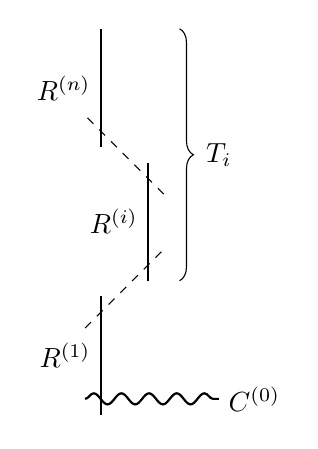
\begin{tikzpicture}
  \draw[thick,decorate,decoration={snake,amplitude=2pt}] (-.2,.2) -0 (1.5,.2);
  \node[right] at (1.5,.2) {$C^{(0)}$};
  \draw[thick] (0,0) -- node[left]{$R^{(1)}$} (0,1.5);
  \draw[dashed] (-.2,1.1) -- (.8,2.1);
  \draw[thick] (.6,1.7) -- node[left]{$R^{(i)}$} (.6,3.2);
  \draw[dashed] (.8,2.8) -- (-.2,3.8);
  \draw[thick] (0,3.4) -- node[left]{$R^{(n)}$} (0,4.9);
  \draw [decorate,decoration={brace,amplitude=5pt,mirror}] (1,1.7) -- (1,4.9) node [midway,xshift=.5cm]{$T_i$};
 \end{tikzpicture}
\end{center}

Because the moduli space $\mathfrak{Pic}_{g,n}^{d,\text{st}}$ is smooth, a general one-parameter family inside this stack will give us a smoothing of our curve. The total space of such a family is a normal surface $S$; thus we can compute the degree of the restriction of $\mathcal M$ to the irreducible components of the central fiber of this family by first restricting $\mathcal M$ to $S$, and then using the intersection theory of the normal surface $S$.

Notice first that $T^\delta|_S = T_{i_\delta}$ where $i_\delta$ is the unique value of $i$ such that
\begin{equation*} \delta = \sum_{j=i_{\delta}}^n e_i \end{equation*}
and if no such $i_\delta$ exists then $T^\delta|_S = 0$. Thus we obtain:
\begin{equation*} \otimes_{0<\delta\leq d}\mathcal{O}_{\mathfrak{C}_{\mathfrak{Pic}}}((\delta-1) T^\delta)|_S = \mathcal{O}_S(\Sigma_{j=1}^n \epsilon_j T_j) \end{equation*}
Now, $R^{(i)}$ has self-intersection $-2$ for $i=1,\ldots,n-1$, and so we have
\begin{equation*}
R^{(i)}\cdot T_j =
  \begin{cases}
    0 & \text{for } j<i \\
    -1 & \text{for } j=i \\
    1 & \text{for } j=i+1 \\
    0 & \text{for } j>i+1
  \end{cases}
\end{equation*}
from which it follows that:
\begin{equation*} \deg \mathcal{M}|_{R^{(i)}} = \deg \mathcal{L}|_{R^{(i)}} - \epsilon_i + \epsilon_{i+1} = e_i - e_i = 0 \end{equation*}
On the other hand $R^{(n)}$ has self-intersection $-1$ and so we have
\begin{equation*}
R^{(n)} \cdot T_j =
\begin{cases}
0 & \text{for } j < n \\
-1 & \text{for } j = n
\end{cases}
\end{equation*}
which implies:
\begin{equation*} \deg \mathcal{M}|_{R^{(n)}} = \deg \mathcal{L}|_{R^{(n)}} - 1 - \epsilon_n = e_n - 1 - (e_n-1) = 0\end{equation*}
Here we have used the fact that $\omega_\pi(\Sigma_i x_i)$ has degree $0$ on $R^{(i)}$ for $i=1,\ldots,n-1$ and degree $-1$ on $R^{(n)}$. Thus $\mathcal{M}$ is trivial on every component on every rational tail, as claimed. The fact that it is $\pi$-relatively ample on the rest of the curve follows from the stability condition and the fact that $\OO_{\mathfrak{C}_{\mathfrak{Pic}}}(T^\delta)$ is effective when restricted to $C^{(0)}$.

In the above discussion we restricted ourselves to the simple case where $R$ is a chain of $\PP^1$s. In general $R$ can be an arbitrary tree of $\PP^1$s. The argument is similar, though combinatorially more complex. For brevity we will discuss one example:

[FIGURE]

Here $R$ has $3$ irreducible components $R^{(0)},R^{(1)},R^{(2)}$ with degrees $e_0,e_1,e_2$ respectively. Let $e = e_0+e_1+e_2$ be the total degree of the rational tail.

Of the divisors $T^{\delta}$ for $0<\delta\leq d$, the total space $S$ only intersects\footnote{Notice in particular that $S$ does not intersect $T^{e_0}$ or $T^{e_0+e_1}$ (unless $e_0=0$).} $T^{e_1}, T^{e_2}$ and $T^e$. We have:
\begin{align*}
T^{e_1}|_S & = R^{(1)} \\
T^{e_2}|_S & = R^{(2)} \\
T^e|_S & = R = R^{(0)} + R^{(1)} + R^{(2)}
\end{align*}
Let us first look at $R^{(1)}$. This has self-intersection $-1$ and so:
\begin{equation*} R^{(1)} \cdot T^{e_1}|_S = -1 \qquad R^{(1)} \cdot T^{e_2}|_S = 0 \qquad R^{(1)} \cdot T^e|_S = 1-1 = 0 \end{equation*}
Thus we obtain
\begin{equation*} \deg \mathcal{M}|_{R^{(1)}} = \deg \mathcal{L}|_{R^{(1)}} - 1 - (e_1 - 1) = 0 \end{equation*}
and same argument applies to $R^{(2)}$. On the other hand, $R^{(0)}$ has self-intersection $-3$ (in general, a component that appears with $n$ adjacent components will have self-intersection $-n$). We have
\begin{equation*} R^{(0)} \cdot T^{e_1}|_S = 1 \qquad R^{(0)} \cdot T^{e_2}|_S = 1 \qquad R^{(0)} \cdot T^e|_S = -3 + 1 + 1 = -1 \end{equation*}
and thus we obtain
\begin{align*} \deg \mathcal{M}|_{R^{(0)}} & = \deg \mathcal{L}|_{R^{(0)}} + 1 + (e_1 - 1) + (e_2 - 1) - (e-1) \\
& = e_0 + e_1 + e_2 - e = 0 \end{align*}
as required.

To summarise, then: we have constructed a line bundle $\mathcal{M}$ on $\mathfrak{C}_{\mathfrak{Pic}}$ which is trivial on the components that we wish to contract and $\pi$-relatively ample elsewhere. By taking the relative Proj construction we therefore obtain another curve
\begin{equation*} \hat{\mathfrak{C}}_{\mathfrak{Pic}}:=\underline{\operatorname{Proj}}_{\mathfrak{Pic}_{g,n}^{d,\operatorname{st}}} \left(\bigoplus_{k\geq 0}\pi_*\mathcal M^{\otimes k}\right) \end{equation*}
over $\mathfrak{Pic}_{g,n}^{d,\text{st}}$, and a map $\rho$ which contracts the rational tails
\bcd
\mathfrak C_{\mathfrak{Pic}}\ar[r,"\rho"]\ar[dr,"\pi" left=3pt] & \hat{\mathfrak{C}}_{\mathfrak{Pic}} \ar[d,"\hat{\pi}"]\\
 & \mathfrak{Pic}_{g,n}^{d,\text{st}}
\ecd
The map $\hat{\pi}$ is flat since it is a family of genus $g$ curves over a reduced base. Furthermore, it can be checked using cohomology and base-change \cite[Theorem 12.11]{HAR} \cite[Corollary 1.5]{Knudsen} (notice that the fibers of $\rho$ are either points or rational curves) that
\begin{equation*}\hat{\mathcal L}:=\rho_*\left(\mathcal L\otimes \bigotimes_{0<\delta\leq d}\mathcal{O}_{\hat{\mathfrak{C}}_{\mathfrak{Pic}}}(\delta T^\delta)\right) \end{equation*}
is a line bundle on $\hat{\mathfrak{C}}_{\mathfrak{Pic}}$ of degree $d$ relative to $\hat{\pi}$. By the Yoneda lemma we thus obtain a comparison morphism $\tilde{\comp}$ fitting into a commutative diagram:
\bcd
\mathfrak C_{\mathfrak{Pic}}\ar[r,"\rho"]\ar[dr,"\pi" left=3pt] & \hat{\mathfrak{C}}_{\mathfrak{Pic}} \ar[d,"\hat{\pi}"]\ar[dr,phantom,"\square" right=-0.5pt]\ar[r] & \mathfrak C_{\mathfrak{Pic}}\ar[d,"\pi"] \\
 & \mathfrak{Pic}_{g,n}^{d,\text{st}}\ar[r,"\tilde{\comp}"] & \mathfrak{Pic}_{g,n}^{d,\text{st}}
\ecd
This discussion all took place at the level of Picard stacks. However the same arguments carry through to give the comparison morphism:
\begin{equation*} \comp\colon \M{g}{n}{\PP^N}{d}\to\Q{g}{n}{\PP^N}{d} \end{equation*}
We have a commutative diagram
\bcd
\M{g}{n}{\PP^N}{d} \ar[d,"\nu_{\mathcal M}"]\ar[r,"\comp"] & \Q{g}{n}{\PP^N}{d}\ar[d,"\nu_{\mathcal Q}"] \\
\mathfrak{Pic}_{g,n}^{d,\text{st}}\ar[r,"\tilde{\comp}"] & \mathfrak{Pic}_{g,n}^{d,\text{st}}
\ecd
and, as before, a diagram of universal curves:
\bcd
\mathcal C_{\mathcal M}\ar[r,"\rho"] \ar[rd,"\pi_{\mathcal M}" left=3pt] & \hat{\mathcal{C}}_{\mathcal{M}}=\comp^*\mathcal C_{\mathcal Q} \ar[d,"\hat{\pi}_{\mathcal{M}}"]\ar[dr,phantom,"\square"]\ar[r] & \mathcal C_{\mathcal Q}\ar[d,"\pi_{\mathcal Q}"] \\
 & \M{g}{n}{\PP^N}{d}\ar[r,"\comp"] & \Q{g}{n}{\PP^N}{d}
\ecd

\subsection{The comparison morphism preserves the virtual classes}
The virtual classes are preserved by the comparison morphism, that is:
\begin{equation*} \comp_* \virt{\M{g}{n}{\PP^N}{d}} = \virt{\Q{g}{n}{\PP^N}{d}} \end{equation*}
The idea, following \cite{Manolache-Push}, is to construct a relative perfect obstruction theory
\begin{equation*} \mathbf{E}_{\comp} \to \mathbf{L}_{\comp} \end{equation*}
for the morphism $\comp$. The construction is best outlined in the arXiv version of \cite[Remark 5.20]{Manolache-Push}. Let $\tilde{\nu}_{\mathcal{M}}$ denote the composition:
\bcd
\M{g}{n}{\PP^N}{d} \ar[r,"\nu_{\mathcal{M}}"] \ar[rr,"{\tilde{\nu}}_{\mathcal{M}}", bend right] & \mathfrak{Pic}_{g,n}^{d,\operatorname{st}} \ar[r,"\tilde{\comp}"] & \mathfrak{Pic}_{g,n}^{d,\operatorname{st}}
\ecd
We may endow this morphism with a relative perfect obstruction theory via the following morphism of exact triangles:
\bcd
\nu_\mathcal M^*\mathbf L_{\tilde{\comp}}\ar[d]\ar[r] & \mathbf E_{\tilde{\nu}_{\mathcal{M}}} \ar[d]\ar[r] & \mathbf E_{\nu_\mathcal M} \ar[d]\ar[r,"{[1]}"] & {}\\
\nu_\mathcal M^*\mathbf L_{\tilde{\comp}}\ar[r] & \mathbf L_{\tilde{\nu}_{\mathcal{M}}} \ar[r] & \mathbf L_{\nu_\mathcal M} \ar[r,"{[1]}"] & {}
\ecd
Notice that $\tilde{\comp}$ is a morphism between smooth Artin stacks. As such we can examine the exact triangle of cotangent complexes induced by $\tilde{\comp}$ and conclude that $\mathbf{L}_{\tilde{\comp}}$ is supported in $[-1,1]$. It then follows easily  that $\mathbf E_{\tilde{\nu}_{\mathcal{M}}}$ is also supported in $[-1,1]$; in order to show that it is perfect, we consider the long exact cohomology sequence near $\h^1(\mathbf E_{\tilde{\nu}_{\mathcal{M}}})$:
\begin{equation*} \h^{0}(\mathbf E_{\nu_\mathcal M}) \to \h^{1}(\nu_\mathcal M^*\mathbf L_{\tilde{\comp}}) \to \h^{1} (\mathbf E_{\tilde{\nu}_{\mathcal{M}}}) \to 0 \end{equation*}
We must show that the morphism $\h^0 (\mathbf{E}_{\nu_{\mathcal{M}}}) \to \h^1(\nu_{\mathcal{M}}^* \mathbf{L}_{\tilde{\comp}})$ is surjective. Looking at the dual picture, we see that the map
\begin{equation*} \h^{1}(\nu_\mathcal M^*\mathbf{L}_{\tilde{\comp}})^\vee \to \h^{0}(\mathbf E_{\nu_\mathcal M})^\vee \cong \h^{0}(\mathbf{L}_{\nu_\mathcal M})^\vee \end{equation*}
is injective, because every infinitesimal automorphism of the rational tail induces a nontrivial deformation of the stable map, since the degree of the stable map is positive on every component of the rational tail. We conclude that $\h^{1}\mathbf E_{\tilde{\nu}_{\mathcal{M}}}=0$ and so indeed $\mathbf{E}_{\tilde{\nu}_{\mathcal{M}}}$ is a perfect obstruction theory for $\tilde{\nu}_{\mathcal{M}}$. It induces the usual virtual fundamental class on the moduli space of stable maps.

Now, we can construct a morphism of obstruction theories (see 
\cite[Lemma 4.19]{Manolache-Push})
\begin{equation*} \comp^*\mathbf E_{\nu_\mathcal Q}\to\mathbf E_{\nu_\mathcal M} \end{equation*}
as follows. We have
\begin{align*} \mathbf E^\vee_{\nu_\mathcal M}& =\R\pi_{\mathcal{M}*}\mathcal L^{\oplus N+1}=\R\hat\pi_* \rho_*\mathcal L^{\oplus N+1} \\
\comp^*\mathbf E^\vee_{\nu_\mathcal Q} & = \chi^* \R \pi_{\mathcal{Q}} \hat{\mathcal{L}}^{\oplus{N+1}} = \R {\hat{\pi}}_{\mathcal{M}*}\hat{\mathcal L}^{\oplus N+1}\end{align*}
where $\hat{\mathcal L}=\rho_*\left(\mathcal L\otimes \bigotimes_{0<\delta\leq d}\mathcal O_{\mathfrak C}(\delta T^\delta)\right)$. Thus $\mathbf E^\vee_{\nu_\mathcal M}\to\comp^*\mathbf E^\vee_{\nu_\mathcal Q}$ comes from the following inclusion of line bundles on $\mathcal C_\mathcal M$:
\[
\mathcal L\hookrightarrow \mathcal L\otimes \bigotimes_{0<\delta\leq d}\mathcal O_{\mathfrak C}(\delta T^\delta).
\]
We now claim that this morphism factors through $\mathbf E_{\tilde{\nu}_{\mathcal{M}}}$. Examining the diagram:
\bcd
& \comp^*\mathbf E_{\nu_\mathcal Q}\ar[dl,dashed,"\exists ?"]\ar[d]\ar[dr,"\phi"] & \\
\mathbf E_{\tilde{\nu}_{\mathcal{M}}} \ar[r] & \mathbf E_{\nu_\mathcal M}\ar[r] & \nu_\mathcal M^*\mathbf L_{\tilde{\comp}}[1] \ar[r,"{[1]}"] & \,
\ecd
we see that it is equivalent to show that $\phi$ is the zero map. This follows formally from the following factorisation:
\bcd
 & & \mathbf L_\comp \ar[ld,"{[1]}" swap] & & \\
\comp^* \mathbf E_{\nu_\mathcal Q}\ar[dd]\ar[r] & \comp^*\mathbf L_{\nu_\mathcal Q}\ar[rr] &  & \mathbf L_{\tilde{\nu}_{\mathcal{M}}}\ar[ul]\ar[dd] & \\
 & & & & \nu_{\mathcal M}^*\mathbf L_{\tilde{\comp}}[1]\ar[ul,"{[1]}" swap] \\
\mathbf E_{\nu_\mathcal M} \ar[rrr] & & & \mathbf L_{\nu_\mathcal M}\ar[ur] & {}
\ecd
We thus obtain a morphism
\begin{equation*} \psi \colon \comp^* \mathbf{E}_{\nu_{\mathcal{Q}}} \to \mathbf{E}_{\tilde{\nu}_{\mathcal{M}}} \end{equation*}
and the cone $C(\psi)$ gives a relative obstruction theory for the comparison morphism $\chi$. A priori, it is supported in $[-2,0]$. By the octahedral axiom we have:
%-------------
\begin{comment}
\begin{center}
\begin{tikzcd}[execute at end picture={
    \begin{scope}[on background layer]
    \fill[pattern=north east lines, pattern color=gray!20] (a.north west) -- (b.north east) -- (b.south east) -- (a.south west) -- cycle;
    \fill[pattern=north west lines, pattern color=gray!20] (c.north west) -- (c.north east) -- (d.south east) -- (d.south west) -- cycle;
    \end{scope}
  }]
\comp^* \mathbb E_{\nu_\mathcal Q}\ar[d]\ar[r] & |[alias=a]| \comp^*\mathbb L_{\nu_\mathcal Q}\ar[r] & |[alias=c]|\mathbb L_{\tilde{\nu}_{\mathcal{M}}}\ar[r]\ar[d] & |[alias=b]| \mathbb L_\comp \\
\mathbb E_{\nu_\mathcal M} \ar[rr] & & \mathbb L_{\nu_\mathcal M}\ar[d] & \\
 & & |[alias=d]| \nu_{\mathcal M}^*\mathbb L_{\comp '}[1]
\end{tikzcd}
\end{center} 
\end{comment}
\begin{comment}
Dually, we look at $\nu_\mathcal M^*\mathbb T_{\tilde{\comp}}[-1]\xrightarrow{\phi^\vee} \R\hat\pi_*(\hat{\mathcal L}^{\oplus r+1})$. Notation: call $R$ the rational tail, joined at the rest of the curve (which we denote by $(C^{(0)},\mathbf p)$ as a marked curve), at the node $q$, which we may occasionally think of as a (smooth) point on $C^{(0)}$. We claim that:
\begin{itemize}
 \item $h^0(\phi^\vee)$ is zero because: the LHS involves automorphisms of the rational tail that leave $C^{(0)}$ fixed, while the RHS involves deformations of $C^{(0)}$, so there is no possible interference.
 \item $h^1(\phi^\vee)$ is zero because: \textcolor{red}{this is slightly awkward.} There are two types of possible contributions to the LHS. They correspond to either moving the node $q$ along $C^{(0)}$, or smoothing it. The former appears in the relative tangent of $\chi'$ only if the marked curve $(C^{(0)},\mathbf p)$ has no automorphisms that may ``move $q$ back'', i.e. $(C^{(0)},\mathbf p)$ is a stable pointed curve. The latter matters only if $(C^{(0)},q,\mathbf p)$ has no moduli, i.e. $(C^{(0)},\mathbf p)$ is a rational tail with less than 3 markings. \textcolor{red}{I will try to justify why the first type vanishes under $h^1(\phi^\vee)$, and leave the second type because I do not understand it as yet.} Look at the long exact sequence
\begin{align*}
  0 &\to \Hom(\Omega_{C^{(0)}},\mathcal O_{C^{(0)}}(-q-\sum p_i)) &\to \Hom(\Omega_{C^{(0)}},\mathcal O_{C^{(0)}}(-\sum p_i)) &\to \\
  T_{C^{(0)},q} &\to \Ext^1(\Omega_{C^{(0)}},\mathcal O_{C^{(0)}}(-q-\sum p_i)) &\to \Ext^1(\Omega_{C^{(0)}},\mathcal O_{C^{(0)}}(-\sum p_i)) &\to 0
 \end{align*}
We are interested in what happens to
\[
 \frac{T_{C^{(0)},q}}{\operatorname{Im}\left( \Hom(\Omega_{C^{(0)}},\mathcal O_{C^{(0)}}(-\sum p_i)) \right)}
\]
under $h^1(\phi^\vee)$. If we can show that $h^1(\phi^\vee)$ factors through $\Ext^1(\Omega_{C^{(0)}},\mathcal O_{C^{(0)}}(-\sum p_i))$ we are in business. Indeed the natural maps
\bcd
\Def_L\ar[d]\ar[r] & \Def_{(C,L)}\ar[d]\ar[r] & \Def_C\ar[d] \\
H^1(\mathcal O_C)\ar[r] & H^1(L^{\oplus r+1})\ar[r] & H^1(f^*T_{\PP^N})
\ecd
show that $h^1(\phi^\vee)$ factors through
\[
\Ext^1(\Omega_{C^{(0)}},\mathcal O_{C^{(0)}}(-q-\sum p_i))\to \Ext^1(\Omega_{C^{(0)}},\mathcal O_{C^{(0)}})\to \Ext^1(f^*\Omega_{\PP^N},\mathcal O_{C^{(0)}})\simeq H^1(f^*T_{\PP^N}).
\]
 \item $h^2(\phi^\vee)$ is zero because: $\mathbb E^\vee_{\tilde{\nu}_{\mathcal{M}}}$ is supported in $[0,1]$.
\end{itemize}
\end{comment}
%----------------------
\begin{center}
 \begin{tikzcd}[cramped]
  \comp^*\mathbf E_{\nu_\mathcal{Q}} \ar[dd,"\psi"]\ar[rrdd,"\tilde{\psi}"] & & & & & & \\
& & & & & & \\
\mathbf E_{\tilde{\nu}_\mathcal{M}}\ar[dd]\ar[rr] & & \mathbf E_{\nu_\mathcal{M}} \ar[rrrr]\ar[dr] & & & & \nu_{\mathcal M}^*\mathbf L_{\tilde{\comp}}{[1]} \\
& & & C(\tilde{\psi})\ar[urrr] & & & \\
C(\psi) \ar[urrr] & & & & & & 
 \end{tikzcd}
\end{center}

Now, $C(\psi)$ is supported in $[-1,0]$ \cite[Lemma 4.20]{Manolache-Push} and $\nu_{\mathcal M}^*\mathbf L_{\tilde{\comp}}{[1]}$ is supported in degrees $[-2,0]$, from which it follows that $C(\psi)=\mathbf E_{\comp}$ is a perfect obstruction theory. The conclusion, that
\begin{equation*} \comp_*\virt{\M{g}{n}{\PP^N}{d}}=\virt{\Q{g}{n}{\PP^N}{d}} \end{equation*}
follows from the connectedness of $\M{g}{n}{\PP^N}{d}$ \cite{KP}, hence of $\Q{g}{n}{\PP^N}{d}$, and an application of the virtual push-forward theorem \cite[Proposition 4.21]{Manolache-Push}.

\subsection{An example where the comparison morphism fails to exist}
We will now explain with an example the reason why a naive attempt to extend the comparison morphism to a general toric variety fails. The problem boils down to the fact that not all toric divisors are nef: a rational tail contained in a such divisor may have a corresponding line bundle with negative degree $-d$; when contracting such a rational tail, we take the line bundle $L(-dq)$, but it is not clear what to do with the sections. We would like to divide them by $z^d$, where $z$ is a local coordinate around $q$, but we are by no means guaranteed that this is possible. Put differently, we now have an inclusion $L|_{C^{(0)}}(-dq)\hookrightarrow L|_{C^{(0)}}$, but the given sections of $L$ do not necessarily live in the image of $H^0(C^{(0)},L|_{C^{(0)}}(-dq))\to H^0(C^{(0)},L|_{C^{(0)}})$.

A concrete example can be found by looking at the Hirzebruch surface $\mathbb F_1=\operatorname{Bl}_{\pt}\PP^1$.
\begin{figure}[h]
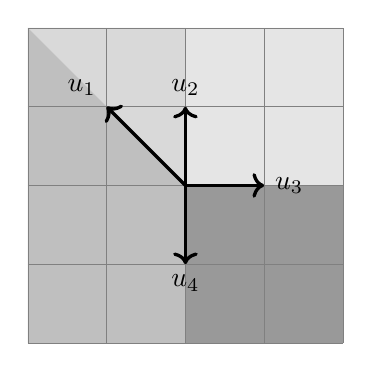
\begin{tikzpicture}
\path [fill=black!10!white] (0,0) -- (2,0) -- (2,2) -- (0,2) -- (0,0);
\path [fill=black!15!white] (0,0) -- (-2,2) -- (0,2) -- (0,0);
\path [fill=black!25!white] (0,0) -- (-2,2) -- (-2,-2) -- (0,-2) -- (0,0);
\path [fill=black!40!white] (0,0) -- (0,-2) -- (2,-2) -- (2,0) -- (0,0);
\draw [help lines] (-2,-2) grid (2,2);
\draw [->,very thick] (0,0) -- (-1,1) node[above left]{$u_1$};
\draw [->,very thick] (0,0) -- (0,1) node[above]{$u_2$};
\draw [->,very thick] (0,0) -- (1,0) node[right]{$u_3$};
\draw [->,very thick] (0,0) -- (0,-1) node[below]{$u_4$};
\end{tikzpicture}
\caption{Toric fan for $\mathbb F_1$.}
\end{figure}

\begin{figure}
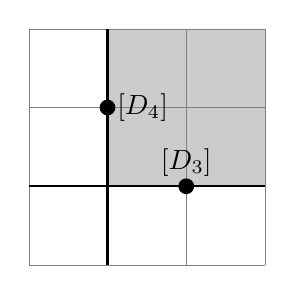
\begin{tikzpicture}
\path [fill=black!20!white] (0,0) -- (2,0) -- (2,2) -- (0,2) -- (0,0);
\draw [help lines] (-1,-1) grid (2,2);
\fill [black] (0,1) circle[radius=.1] node[right]{${[D_4]}$};
\fill [black] (1,0) circle[radius=.1] node[above]{${[D_3]}$};
\draw [thick] (-1,0) -- (2,0);
\draw [thick] (0,-1) -- (0,2);
\end{tikzpicture}
\caption{Nef cone $\operatorname{Nef}(\mathbb F_1)$.}
\end{figure}

\begin{figure}
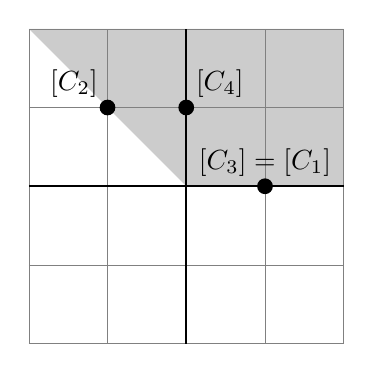
\begin{tikzpicture}
\path [fill=black!20!white] (0,0) -- (2,0) -- (2,2) -- (-2,2) -- (0,0);
\draw [help lines] (-2,-2) grid (2,2);
\fill [black] (0,1) circle[radius=.1] node[above right]{${[C_4]}$};
\fill [black] (1,0) circle[radius=.1] node[above]{${[C_3]}={[C_1]}$};
\fill [black] (-1,1) circle[radius=.1] node[above left]{${[C_2]}$};
\draw [thick] (-2,0) -- (2,0);
\draw [thick] (0,-2) -- (0,2);
\end{tikzpicture}
\caption{Mori cone $\overline{\operatorname{NE}}(\mathbb F_1)$.}
\end{figure}

The group $\Pic(\mathbb F_1)$ is generated by $D_3$ and $D_4$, with relations $D_1=D_3$ and $D_2=D_4-D_3$; the intersection form is given by
\[
{}
\begin{cases}
 D_3^2=0 \\
 D_3\cdot D_4=0 \\
 D_4^2=1
\end{cases} 
\]
When thinking of $\mathbb F_1$ as a $\PP^1$-bundle over $\PP^1$, $C_1$ and $C_3$ represent the fibers of the bundle (over the toric points of $\PP^1$), while $C_4$ (resp. $C_2$) is the zero/positive (resp. infinity/negative) section; when thinking of $\mathbb F_1$ as $\operatorname{Bl}_{p}\PP^1$, $C_2$ is the exceptional divisor, $C_4$ is the toric line not passing through $p$, and $C_1,C_3$ are the strict transforms of the toric lines through $p$.

Let us look at $\M{0}{2}{\mathbb F_1}{[C_4]}$. Since $[C_4]=[C_2]+[C_3]$, there are going to be maps of the following sort: the source curve is reducible $R_1\sqcup_q R_2$, $R_1$ is mapped isomorphically to a fiber (i.e. in class $[C_3]$) and $R_2$ is mapped isomorphically to $C_2$, all the markings belong to $R_1$. So $R_2$ is a rational tail and deserves to be contracted. Notice that the line bundle $\mathcal O(D_2)$ has degree $-1$ on $R_2$ (and $1$ on $R_1$). In this case everything works well because the corresponding section $u_{2|R_1}$ must vanish at the node, so we can divide it by a chosen (once for all toric line bundles) section of $\mathcal O_{R_1}(q)$.

Consider now $\M{0}{2}{\mathbb F_1}{2[C_2]+[C_3]}$. Certainly there are going to be maps similar to the ones described above, with $R_2$ now covering $C_2$ $2\colon 1$. The point is that $\mathcal O(D_2)$ has degree $-2$ on $R_2$, but $u_{2|R_1}$ doesn't have to vanish at the node of order $2$, so we are in trouble. 
\begin{comment}

\textcolor{blue}{Something is going on here: in this case there is a boundary component where the map is of the type that we have just described, and the requirement that $u_{2|R_1}$ vanishes of order $2$ at the node defines precisely the intersection with the main component. Check this. Could we possibly exploit this phenomenon to define a smaller compactification, possibly even smaller than quasimaps?} 

\end{comment}

\section{The Quasimap String Equation for $\PP^r$}

The string equation for the Gromov--Witten invariants of a smooth projective variety $X$ is given by
\begin{align*} \langle \mathbbm{1} , \gamma_1 \psi^{a_1} , \ldots, & \gamma_n \psi^{a_n} \rangle_{g,n+1,\beta}^X = \\
&  \sum_{i=1}^n \langle \gamma_1 \psi^{a_1}, \ldots, \gamma_{i-1} \psi^{a_{i-1}} , \gamma_i \psi^{a_i - 1} , \gamma_{i+1} \psi^{a_{i+1}} \ldots, \gamma_n \psi^{a_n} \rangle_{g,n,\beta}^X \end{align*}
where $\mathbbm{1} \in H^*(X)$ is the unit class (by convention any term involving a negative power of $\psi$ is set to zero). Since Gromov--Witten invariants and quasimap invariants coincide for $X=\PP^r$ (\cite[Section 5.4]{Manolache-Push}) we know that the same equation holds for quasimap invariants to $\PP^r$.

Nevertheless, it would be illuminating to have a direct proof of this statement, without relying on the equivalence with Gromov--Witten theory. Amongst other things, such a proof would necessarily involve some nontrivial intersection computations in the cohomology ring of the quasimap space, which would be of independent interest.

The proof of the classical string equation (for Gromov--Witten invariants) relies on three key lemmas involving certain codimension--1 classes on the moduli space of stable maps. Let
\begin{equation*} \pi : \M{g}{n+1}{X}{\beta} \to \M{g}{n}{X}{\beta}\end{equation*}
denote the contraction map given by forgetting the last marked point and stabilising. Then we have:

\begin{enumerate}
\item $\psi_i = \pi^* \psi_i + D_{i,n+1}$
\item $\psi_i \cdot D_{i,n+1} = 0$
\item $D_{i,n+1} \cdot D_{j,n+1} = 0$ for $i \neq j$
\end{enumerate}

Here $D_{i,n+1}$ is  the locus of stable maps $(C,x_1, \ldots, x_{n+1}, f)$ such that we can split up $C$ into two pieces, $C = C^\prime \cup C^{\prime\prime}$ (intersecting in a single node) such that $C^{\prime\prime}$ has degree $0$ and contains only the markings $x_i$ and $x_{n+1}$.

[FIGURE]

We would like to have some analogue of these results in the quasimap setting. In fact, equations (2) and (3) carry over without difficulty. Equation (1), on the other hand, is rather more delicate.

In the stable map setting, equation (1) is proved by considering the following diagram
\bcd
\mathcal{C}_{g,n+1} \ar[r,"\rho"] \ar[dr, "\psi" below left] & \pi^* \mathcal{C}_{g,n} \ar[r,"\alpha"] \ar[d, "\eta"] & \mathcal{C}_{g,n} \ar[d,"\varphi"] \\
& \M{g}{n+1}{X}{\beta} \ar[r,"\pi"] & \M{g}{n}{X}{\beta}
\ecd
where the square on the right is cartesian. On fibres, the map $\rho$ contracts rational components of $\mathcal{C}_{g,n+1}$ on which $f$ is constant and which contain exactly three special points, one of which is $x_{n+1}$. Thus, we see that
\begin{equation*} \rho^*(x_i) = x_i + R_{i,n+1} \end{equation*}
where $R_{i,n+1} \subseteq C_{g,n+1}$ consists fibrewise of the rational tails containing only $x_i$ and $x_{n+1}$; it is a closed substack of $\psi^{-1}(D_{i,n+1})$ of codimension $0$.

On the other hand, we have (REFERENCE):
\begin{equation*} \rho^* \omega_\eta(\Sigma_{i=1}^n x_i) = \omega_\psi(\Sigma_{i=1}^n x_i) \end{equation*}
Taking Chern classes and combining this with the above result we obtain:
\begin{equation*} \operatorname{c}_1(\rho^* \omega_\eta) = \operatorname{c}_1(\omega_\psi) - \Sigma_{i=1}^n R_{i,n+1} \end{equation*}
We can now pull back along the section $x_i$ and  use the fact that $x_i^* R_{j,n+1} = \delta_{i,j} D_{i,n+1}$ to obtain:
\begin{equation*} \operatorname{c}_1(x_i^*\rho^* \omega_\eta) = \operatorname{c}_1(x_i^* \omega_\psi) - D_{i,n+1} \end{equation*}
Now, $\rho^* \omega_\eta = \rho^* \alpha^* \omega_\varphi$, and so:
\begin{equation*} x_i^* \rho^* \omega_\eta = \pi^* x_i^* \omega_\varphi \end{equation*}
Thus we end up with
\begin{equation*} \pi^*\operatorname{c}_1(x_i^* \omega_\varphi) = \operatorname{c}_1(x_i^* \omega_\psi) - D_{i,n+1} \end{equation*}
which is equation (1) above.

What is different in the case of quasimaps? We have a similar-looking diagram
\bcd
\mathcal{C}_{g,n+1} \ar[r,"\rho"] \ar[dr, "\psi" below left] & \pi^* \mathcal{C}_{g,n} \ar[r,"\alpha"] \ar[d, "\eta"] & \mathcal{C}_{g,n} \ar[d,"\varphi"] \\
& \Q{g}{n+1}{X}{\beta} \ar[r,"\pi"] & \Q{g}{n}{X}{\beta}
\ecd
but now, because of the stronger stability condition, $\rho$ also contracts the locus $T_{n+1}$ consisting of rational tails (of any degree) with a single marking $x_{n+1}$. We claim that:

\begin{conj} $\rho^* \omega_\eta ( \Sigma_{i=1}^n x_i ) = \omega_\psi (\Sigma_{i=1}^n x_i - T_{n+1})$ \end{conj}

Once we have this, the string equation follows as in the stable maps case by pulling back along the section $x_i$ (and using the obvious fact that $x_i^* T_{n+1} = 0$).

\subsection{Comparison with the GIT construction} \label{Section comparison with GIT construction}

In this section we prove the comparison result promised in Remark \ref{GIT comparison remark}

[GENERALISE TO $X$ ANY TORIC VARIETY]
Let $X$ be a hypersurface of degree $a$ in $\PP^r$. In the preceding sections, we have put a virtual class on $\Q{g}{n}{X}{d}$ by way of the following Cartesian diagram:

\bcd
\Q{g}{n}{X}{d}\ar[d]\ar[r] & \Q{g}{n}{\PP^r}{d}\ar[d,"\nu_a"] \\
\Q{g}{n}{H}{ad}\ar[r] & \Q{g}{n}{\PP^N}{ad}
\ecd

where $N={{r+a}\choose{a}}-1$ and $\nu_a$ is the Veronese embedding. In fact, $\Q{g}{n}{X}{d}$ is thought of as representing stable quasimaps to $\PP^r$ such that the corresponding sections satisfy the equation for $X$ inside $\PP^r$, that is a homogeneous polynomial $Q$ of degree $a$, i.e. gives a section of $L^{\otimes a}$ on the source curve $C$.

We wish to compare this with the GIT approach of \cite{CFKM}. Here $X$ is seen as the GIT quotient of the affine cone $C_X\subseteq \mathbb A^{r+1}$ with respect to the diagonal $\mathbb G_m$-action. Objects of $\Q{g}{n}{X}{d}^\text{GIT}$ are diagrams of the form

\bcd
P\ar[d,"\mathbb G_m"]\ar[r] & C_X & \text{or, equivalently,} & P\times_{\mathbb G_m} C_X \ar[d,"\rho" left] \\
C & & & C \ar[u,bend right,"u"right]
\ecd
and the dual perfect obstruction theory with respect to $\mathfrak{Bun}_{\mathbb G_m}$ is given by $R^\bullet\pi_*(u^*\mathbb T^\bullet_\rho$), where $\pi\colon \mathcal C_{\mathfrak{Bun}}\to\mathfrak{Bun}_{\mathbb G_m}$ is the universal curve.

Notice that $\mathfrak{Bun}_{\mathbb G_m}\simeq \mathfrak{Pic}$ by taking the line bundle $L=P\times_{\mathbb G_m}\mathbb A^1\to C$ associated to the $\mathbb G_m$-torsor $P\to C$. Furthermore, the $\mathbb G_m$-equivariant embedding in a smooth stack
\bcd
P\times_{\mathbb G_m} C_X \ar[r,hook]\ar[d,"\rho" left] & P\times_{\mathbb G_m}\mathbb A^{r+1}\simeq L^{\oplus r+1}\ar[dl]\\
C \ar[u,bend right,"u"right] &
\ecd
gives us $u^*T^\bullet_\rho\simeq[L^{\oplus r+1}\to L^{\otimes a}]$, where the arrow is induced by $Q$, and shows that both the modular interpretation and the obstruction theory coincide.

\bibliographystyle{alpha}
\bibliography{relqm}

\end{document}